% Options for packages loaded elsewhere
\PassOptionsToPackage{unicode}{hyperref}
\PassOptionsToPackage{hyphens}{url}
\PassOptionsToPackage{dvipsnames,svgnames,x11names}{xcolor}
%
\documentclass[
  ignorenonframetext,
]{beamer}
\usepackage{pgfpages}
\setbeamertemplate{caption}[numbered]
\setbeamertemplate{caption label separator}{: }
\setbeamercolor{caption name}{fg=normal text.fg}
\beamertemplatenavigationsymbolsempty
% Prevent slide breaks in the middle of a paragraph
\widowpenalties 1 10000
\raggedbottom

\usepackage{amsmath,amssymb}
\usepackage{iftex}
\ifPDFTeX
  \usepackage[T1]{fontenc}
  \usepackage[utf8]{inputenc}
  \usepackage{textcomp} % provide euro and other symbols
\else % if luatex or xetex
  \usepackage{unicode-math}
  \defaultfontfeatures{Scale=MatchLowercase}
  \defaultfontfeatures[\rmfamily]{Ligatures=TeX,Scale=1}
\fi
\usepackage{lmodern}
\usetheme[]{AnnArbor}
\usecolortheme{dolphin}
\usefonttheme{structurebold}
\ifPDFTeX\else  
    % xetex/luatex font selection
\fi
% Use upquote if available, for straight quotes in verbatim environments
\IfFileExists{upquote.sty}{\usepackage{upquote}}{}
\IfFileExists{microtype.sty}{% use microtype if available
  \usepackage[]{microtype}
  \UseMicrotypeSet[protrusion]{basicmath} % disable protrusion for tt fonts
}{}
\makeatletter
\@ifundefined{KOMAClassName}{% if non-KOMA class
  \IfFileExists{parskip.sty}{%
    \usepackage{parskip}
  }{% else
    \setlength{\parindent}{0pt}
    \setlength{\parskip}{6pt plus 2pt minus 1pt}}
}{% if KOMA class
  \KOMAoptions{parskip=half}}
\makeatother
\usepackage{xcolor}
\newif\ifbibliography
\setlength{\emergencystretch}{3em} % prevent overfull lines
\setcounter{secnumdepth}{-\maxdimen} % remove section numbering

\usepackage{color}
\usepackage{fancyvrb}
\newcommand{\VerbBar}{|}
\newcommand{\VERB}{\Verb[commandchars=\\\{\}]}
\DefineVerbatimEnvironment{Highlighting}{Verbatim}{commandchars=\\\{\}}
% Add ',fontsize=\small' for more characters per line
\usepackage{framed}
\definecolor{shadecolor}{RGB}{241,243,245}
\newenvironment{Shaded}{\begin{snugshade}}{\end{snugshade}}
\newcommand{\AlertTok}[1]{\textcolor[rgb]{0.68,0.00,0.00}{#1}}
\newcommand{\AnnotationTok}[1]{\textcolor[rgb]{0.37,0.37,0.37}{#1}}
\newcommand{\AttributeTok}[1]{\textcolor[rgb]{0.40,0.45,0.13}{#1}}
\newcommand{\BaseNTok}[1]{\textcolor[rgb]{0.68,0.00,0.00}{#1}}
\newcommand{\BuiltInTok}[1]{\textcolor[rgb]{0.00,0.23,0.31}{#1}}
\newcommand{\CharTok}[1]{\textcolor[rgb]{0.13,0.47,0.30}{#1}}
\newcommand{\CommentTok}[1]{\textcolor[rgb]{0.37,0.37,0.37}{#1}}
\newcommand{\CommentVarTok}[1]{\textcolor[rgb]{0.37,0.37,0.37}{\textit{#1}}}
\newcommand{\ConstantTok}[1]{\textcolor[rgb]{0.56,0.35,0.01}{#1}}
\newcommand{\ControlFlowTok}[1]{\textcolor[rgb]{0.00,0.23,0.31}{\textbf{#1}}}
\newcommand{\DataTypeTok}[1]{\textcolor[rgb]{0.68,0.00,0.00}{#1}}
\newcommand{\DecValTok}[1]{\textcolor[rgb]{0.68,0.00,0.00}{#1}}
\newcommand{\DocumentationTok}[1]{\textcolor[rgb]{0.37,0.37,0.37}{\textit{#1}}}
\newcommand{\ErrorTok}[1]{\textcolor[rgb]{0.68,0.00,0.00}{#1}}
\newcommand{\ExtensionTok}[1]{\textcolor[rgb]{0.00,0.23,0.31}{#1}}
\newcommand{\FloatTok}[1]{\textcolor[rgb]{0.68,0.00,0.00}{#1}}
\newcommand{\FunctionTok}[1]{\textcolor[rgb]{0.28,0.35,0.67}{#1}}
\newcommand{\ImportTok}[1]{\textcolor[rgb]{0.00,0.46,0.62}{#1}}
\newcommand{\InformationTok}[1]{\textcolor[rgb]{0.37,0.37,0.37}{#1}}
\newcommand{\KeywordTok}[1]{\textcolor[rgb]{0.00,0.23,0.31}{\textbf{#1}}}
\newcommand{\NormalTok}[1]{\textcolor[rgb]{0.00,0.23,0.31}{#1}}
\newcommand{\OperatorTok}[1]{\textcolor[rgb]{0.37,0.37,0.37}{#1}}
\newcommand{\OtherTok}[1]{\textcolor[rgb]{0.00,0.23,0.31}{#1}}
\newcommand{\PreprocessorTok}[1]{\textcolor[rgb]{0.68,0.00,0.00}{#1}}
\newcommand{\RegionMarkerTok}[1]{\textcolor[rgb]{0.00,0.23,0.31}{#1}}
\newcommand{\SpecialCharTok}[1]{\textcolor[rgb]{0.37,0.37,0.37}{#1}}
\newcommand{\SpecialStringTok}[1]{\textcolor[rgb]{0.13,0.47,0.30}{#1}}
\newcommand{\StringTok}[1]{\textcolor[rgb]{0.13,0.47,0.30}{#1}}
\newcommand{\VariableTok}[1]{\textcolor[rgb]{0.07,0.07,0.07}{#1}}
\newcommand{\VerbatimStringTok}[1]{\textcolor[rgb]{0.13,0.47,0.30}{#1}}
\newcommand{\WarningTok}[1]{\textcolor[rgb]{0.37,0.37,0.37}{\textit{#1}}}

\providecommand{\tightlist}{%
  \setlength{\itemsep}{0pt}\setlength{\parskip}{0pt}}\usepackage{longtable,booktabs,array}
\usepackage{calc} % for calculating minipage widths
\usepackage{caption}
% Make caption package work with longtable
\makeatletter
\def\fnum@table{\tablename~\thetable}
\makeatother
\usepackage{graphicx}
\makeatletter
\def\maxwidth{\ifdim\Gin@nat@width>\linewidth\linewidth\else\Gin@nat@width\fi}
\def\maxheight{\ifdim\Gin@nat@height>\textheight\textheight\else\Gin@nat@height\fi}
\makeatother
% Scale images if necessary, so that they will not overflow the page
% margins by default, and it is still possible to overwrite the defaults
% using explicit options in \includegraphics[width, height, ...]{}
\setkeys{Gin}{width=\maxwidth,height=\maxheight,keepaspectratio}
% Set default figure placement to htbp
\makeatletter
\def\fps@figure{htbp}
\makeatother
% definitions for citeproc citations
\NewDocumentCommand\citeproctext{}{}
\NewDocumentCommand\citeproc{mm}{%
  \begingroup\def\citeproctext{#2}\cite{#1}\endgroup}
\makeatletter
 % allow citations to break across lines
 \let\@cite@ofmt\@firstofone
 % avoid brackets around text for \cite:
 \def\@biblabel#1{}
 \def\@cite#1#2{{#1\if@tempswa , #2\fi}}
\makeatother
\newlength{\cslhangindent}
\setlength{\cslhangindent}{1.5em}
\newlength{\csllabelwidth}
\setlength{\csllabelwidth}{3em}
\newenvironment{CSLReferences}[2] % #1 hanging-indent, #2 entry-spacing
 {\begin{list}{}{%
  \setlength{\itemindent}{0pt}
  \setlength{\leftmargin}{0pt}
  \setlength{\parsep}{0pt}
  % turn on hanging indent if param 1 is 1
  \ifodd #1
   \setlength{\leftmargin}{\cslhangindent}
   \setlength{\itemindent}{-1\cslhangindent}
  \fi
  % set entry spacing
  \setlength{\itemsep}{#2\baselineskip}}}
 {\end{list}}
\usepackage{calc}
\newcommand{\CSLBlock}[1]{\hfill\break\parbox[t]{\linewidth}{\strut\ignorespaces#1\strut}}
\newcommand{\CSLLeftMargin}[1]{\parbox[t]{\csllabelwidth}{\strut#1\strut}}
\newcommand{\CSLRightInline}[1]{\parbox[t]{\linewidth - \csllabelwidth}{\strut#1\strut}}
\newcommand{\CSLIndent}[1]{\hspace{\cslhangindent}#1}


% logo
\titlegraphic{
\includegraphics[width=4cm]{../000_logos/logo-blue-vertical}}
\logo{\ifnum\thepage>1
\includegraphics[width=0.5cm]{../000_logos/logo-blue-vertical}\fi}

% UMNG: Manual de image institucional

% Colors

% Umng
\definecolor{yellow}{HTML}{fdc600}
\definecolor{red}{HTML}{ee2a24}

% Estudios a Distancia
\definecolor{blue1}{HTML}{12245b}
\definecolor{blue2}{HTML}{767ca6}
\definecolor{blue3}{HTML}{cad2ec}

% Modify items
\setbeamercolor{palette primary}{bg=blue3}
\setbeamercolor{palette tertiary}{bg=blue1}
\setbeamercolor{frametitle}{bg=yellow}

% Hyperlinks
\hypersetup{
  linkcolor=red,
  citecolor=red
}

\makeatletter
\@ifpackageloaded{caption}{}{\usepackage{caption}}
\AtBeginDocument{%
\ifdefined\contentsname
  \renewcommand*\contentsname{Table of contents}
\else
  \newcommand\contentsname{Table of contents}
\fi
\ifdefined\listfigurename
  \renewcommand*\listfigurename{List of Figures}
\else
  \newcommand\listfigurename{List of Figures}
\fi
\ifdefined\listtablename
  \renewcommand*\listtablename{List of Tables}
\else
  \newcommand\listtablename{List of Tables}
\fi
\ifdefined\figurename
  \renewcommand*\figurename{Figure}
\else
  \newcommand\figurename{Figure}
\fi
\ifdefined\tablename
  \renewcommand*\tablename{Table}
\else
  \newcommand\tablename{Table}
\fi
}
\@ifpackageloaded{float}{}{\usepackage{float}}
\floatstyle{ruled}
\@ifundefined{c@chapter}{\newfloat{codelisting}{h}{lop}}{\newfloat{codelisting}{h}{lop}[chapter]}
\floatname{codelisting}{Listing}
\newcommand*\listoflistings{\listof{codelisting}{List of Listings}}
\makeatother
\makeatletter
\makeatother
\makeatletter
\@ifpackageloaded{caption}{}{\usepackage{caption}}
\@ifpackageloaded{subcaption}{}{\usepackage{subcaption}}
\makeatother

\ifLuaTeX
\usepackage[bidi=basic]{babel}
\else
\usepackage[bidi=default]{babel}
\fi
\babelprovide[main,import]{english}
% get rid of language-specific shorthands (see #6817):
\let\LanguageShortHands\languageshorthands
\def\languageshorthands#1{}
\ifLuaTeX
  \usepackage{selnolig}  % disable illegal ligatures
\fi
\usepackage{bookmark}

\IfFileExists{xurl.sty}{\usepackage{xurl}}{} % add URL line breaks if available
\urlstyle{same} % disable monospaced font for URLs
\hypersetup{
  pdftitle={Reducing Data Complexity},
  pdfauthor={Luis Francisco Gómez López},
  pdflang={en},
  colorlinks=true,
  linkcolor={Maroon},
  filecolor={Maroon},
  citecolor={Blue},
  urlcolor={Blue},
  pdfcreator={LaTeX via pandoc}}


\title{Reducing Data Complexity}
\author{Luis Francisco Gómez López}
\date{2024-09-18}
\institute{FAEDIS}

\begin{document}
\frame{\titlepage}

\renewcommand*\contentsname{Table of contents}
\begin{frame}[allowframebreaks]
  \frametitle{Table of contents}
  \tableofcontents[hideallsubsections]
\end{frame}

\section{Please Read Me}\label{please-read-me}

\begin{frame}{}
\phantomsection\label{section}
\begin{itemize}
\tightlist
\item
  This presentation is based on (\citeproc{ref-chapman_r_2019}{Chapman
  and Feit 2019, chap. 8})
\end{itemize}
\end{frame}

\section{Purpose}\label{purpose}

\begin{frame}{}
\phantomsection\label{section-1}
\begin{itemize}
\tightlist
\item
  Apply data complexity reduction by using the principal component
  analysis technique
\end{itemize}
\end{frame}

\section{Consumer brand perception
survey}\label{consumer-brand-perception-survey}

\begin{frame}[fragile]{}
\phantomsection\label{section-2}
\begin{itemize}
\item
  On a scale from 1 to 10, where 1 is least and 10 is most, how
  \texttt{\textless{}perceptual\ adjective\textgreater{}} is
  \texttt{\textless{}brand\textgreater{}}?
\item
  100 respondents rate 10 brands on 9 perceptual adjectives

  \begin{itemize}
  \tightlist
  \item
    \textbf{perform}: has strong performance \((1, 2, \ldots, 10)\)
  \item
    \textbf{leader}: is a leader in the field \((1, 2, \ldots, 10)\)
  \item
    \textbf{latest}: has the latest products \((1, 2, \ldots, 10)\)
  \item
    \textbf{fun}: is fun \((1, 2, \ldots, 10)\)
  \item
    \textbf{serious}: is serious \((1, 2, \ldots, 10)\)
  \item
    \textbf{bargain}: products are a bargain \((1, 2, \ldots, 10)\)
  \item
    \textbf{value}: products are a good value \((1, 2, \ldots, 10)\)
  \item
    \textbf{trendy}: is trendy \((1, 2, \ldots, 10)\)
  \item
    \textbf{rebuy}: I would buy from
    \texttt{\textless{}brand\textgreater{}} again \((1, 2, \ldots, 10)\)
  \item
    \textbf{brand}: coffee brand rated by a consumer
    \((a, b, \ldots, j)\)
  \end{itemize}
\end{itemize}
\end{frame}

\begin{frame}[fragile]{}
\phantomsection\label{section-3}
\begin{itemize}
\tightlist
\item
  Import data
\end{itemize}

\tiny

\begin{Shaded}
\begin{Highlighting}[]
\NormalTok{consumer\_brand }\OtherTok{\textless{}{-}} \FunctionTok{read\_csv}\NormalTok{(}\StringTok{"http://goo.gl/IQl8nc"}\NormalTok{)}
\NormalTok{consumer\_brand }\SpecialCharTok{|\textgreater{}} \FunctionTok{head}\NormalTok{(}\AttributeTok{n =} \DecValTok{5}\NormalTok{)}
\end{Highlighting}
\end{Shaded}

\begin{verbatim}
# A tibble: 5 x 10
  perform leader latest   fun serious bargain value trendy rebuy brand
    <dbl>  <dbl>  <dbl> <dbl>   <dbl>   <dbl> <dbl>  <dbl> <dbl> <chr>
1       2      4      8     8       2       9     7      4     6 a    
2       1      1      4     7       1       1     1      2     2 a    
3       2      3      5     9       2       9     5      1     6 a    
4       1      6     10     8       3       4     5      2     1 a    
5       1      1      5     8       1       9     9      1     1 a    
\end{verbatim}
\end{frame}

\begin{frame}[fragile]{}
\phantomsection\label{section-4}
\begin{itemize}
\tightlist
\item
  Transform data
\end{itemize}

\tiny

\begin{Shaded}
\begin{Highlighting}[]
\NormalTok{consumer\_brand\_scale }\OtherTok{\textless{}{-}}\NormalTok{ consumer\_brand }\SpecialCharTok{|\textgreater{}} 
  \FunctionTok{mutate}\NormalTok{(}\FunctionTok{across}\NormalTok{(perform}\SpecialCharTok{:}\NormalTok{rebuy, }
                \AttributeTok{.fns =} \SpecialCharTok{\textasciitilde{}} \FunctionTok{scale}\NormalTok{(}\AttributeTok{x =}\NormalTok{ .x,}
                               \AttributeTok{center =} \ConstantTok{TRUE}\NormalTok{,}
                               \AttributeTok{scale =} \ConstantTok{TRUE}\NormalTok{)[,}\DecValTok{1}\NormalTok{]))}
\NormalTok{consumer\_brand\_scale }\SpecialCharTok{|\textgreater{}} \FunctionTok{head}\NormalTok{()}
\end{Highlighting}
\end{Shaded}

\begin{verbatim}
# A tibble: 6 x 10
  perform leader latest    fun serious bargain  value trendy  rebuy brand
    <dbl>  <dbl>  <dbl>  <dbl>   <dbl>   <dbl>  <dbl>  <dbl>  <dbl> <chr>
1  -0.777 -0.160  0.586  0.704  -0.836  1.78    1.11  -0.445  0.893 a    
2  -1.09  -1.31  -0.713  0.340  -1.20  -1.22   -1.39  -1.17  -0.679 a    
3  -0.777 -0.543 -0.388  1.07   -0.836  1.78    0.276 -1.54   0.893 a    
4  -1.09   0.607  1.24   0.704  -0.476 -0.0971  0.276 -1.17  -1.07  a    
5  -1.09  -1.31  -0.388  0.704  -1.20   1.78    1.94  -1.54  -1.07  a    
6  -0.777  1.37   0.911 -0.389  -0.476  1.40    1.11  -1.54  -0.679 a    
\end{verbatim}
\end{frame}

\begin{frame}[fragile]{}
\phantomsection\label{section-5}
\begin{itemize}
\item
  Summarize data

  \begin{itemize}
  \tightlist
  \item
    Ups the table is really big!!! Try it in your console to see the
    complete table
  \end{itemize}
\end{itemize}

\tiny

\begin{Shaded}
\begin{Highlighting}[]
\NormalTok{consumer\_brand\_scale }\SpecialCharTok{|\textgreater{}} \FunctionTok{skim}\NormalTok{()}
\end{Highlighting}
\end{Shaded}
\end{frame}

\begin{frame}[fragile]{}
\phantomsection\label{section-6}
\begin{itemize}
\item
  Correlation matrices

  \begin{itemize}
  \tightlist
  \item
    Pearson correlation coefficients for samples in a tibble
  \end{itemize}
\end{itemize}

\tiny

\begin{Shaded}
\begin{Highlighting}[]
\NormalTok{correlation\_matrix }\OtherTok{\textless{}{-}}\NormalTok{ consumer\_brand\_scale }\SpecialCharTok{|\textgreater{}} 
  \FunctionTok{select}\NormalTok{(perform}\SpecialCharTok{:}\NormalTok{rebuy) }\SpecialCharTok{|\textgreater{}} 
\NormalTok{  corrr}\SpecialCharTok{::}\FunctionTok{correlate}\NormalTok{(}\AttributeTok{use =} \StringTok{"pairwise.complete.obs"}\NormalTok{, }\CommentTok{\# There are NA values}
                   \AttributeTok{method =} \StringTok{"pearson"}\NormalTok{,}
                   \AttributeTok{diagonal =} \ConstantTok{NA}\NormalTok{)}
\NormalTok{correlation\_matrix }\CommentTok{\# Ups!!! The tibble is wide. Check out the tibble in your console}
\end{Highlighting}
\end{Shaded}

\begin{verbatim}
# A tibble: 9 x 10
  term     perform  leader   latest     fun  serious  bargain   value   trendy
  <chr>      <dbl>   <dbl>    <dbl>   <dbl>    <dbl>    <dbl>   <dbl>    <dbl>
1 perform NA        0.500  -0.122   -0.256   0.359    0.0571   0.102   0.00873
2 leader   0.500   NA       0.0269  -0.290   0.571    0.0331   0.118   0.0665 
3 latest  -0.122    0.0269 NA        0.245   0.00995 -0.254   -0.343   0.628  
4 fun     -0.256   -0.290   0.245   NA      -0.281   -0.0666  -0.145   0.128  
5 serious  0.359    0.571   0.00995 -0.281  NA       -0.00266  0.0238  0.121  
6 bargain  0.0571   0.0331 -0.254   -0.0666 -0.00266 NA        0.740  -0.351  
7 value    0.102    0.118  -0.343   -0.145   0.0238   0.740   NA      -0.435  
8 trendy   0.00873  0.0665  0.628    0.128   0.121   -0.351   -0.435  NA      
9 rebuy    0.307    0.209  -0.397   -0.237   0.181    0.467    0.506  -0.298  
# i 1 more variable: rebuy <dbl>
\end{verbatim}
\end{frame}

\begin{frame}[fragile]{}
\phantomsection\label{section-7}
\begin{itemize}
\item
  Correlation matrices

  \begin{itemize}
  \tightlist
  \item
    Pearson correlation coefficients for samples in a tibble
  \end{itemize}
\end{itemize}

\tiny

\begin{Shaded}
\begin{Highlighting}[]
\NormalTok{correlation\_matrix }\SpecialCharTok{|\textgreater{}} 
  \FunctionTok{autoplot}\NormalTok{(}\AttributeTok{method =} \StringTok{"HC"}\NormalTok{, }\CommentTok{\# Hierarchical clustering: More details in Chapter 11 }
           \AttributeTok{triangular =} \StringTok{"lower"}\NormalTok{)}
\end{Highlighting}
\end{Shaded}

\begin{center}
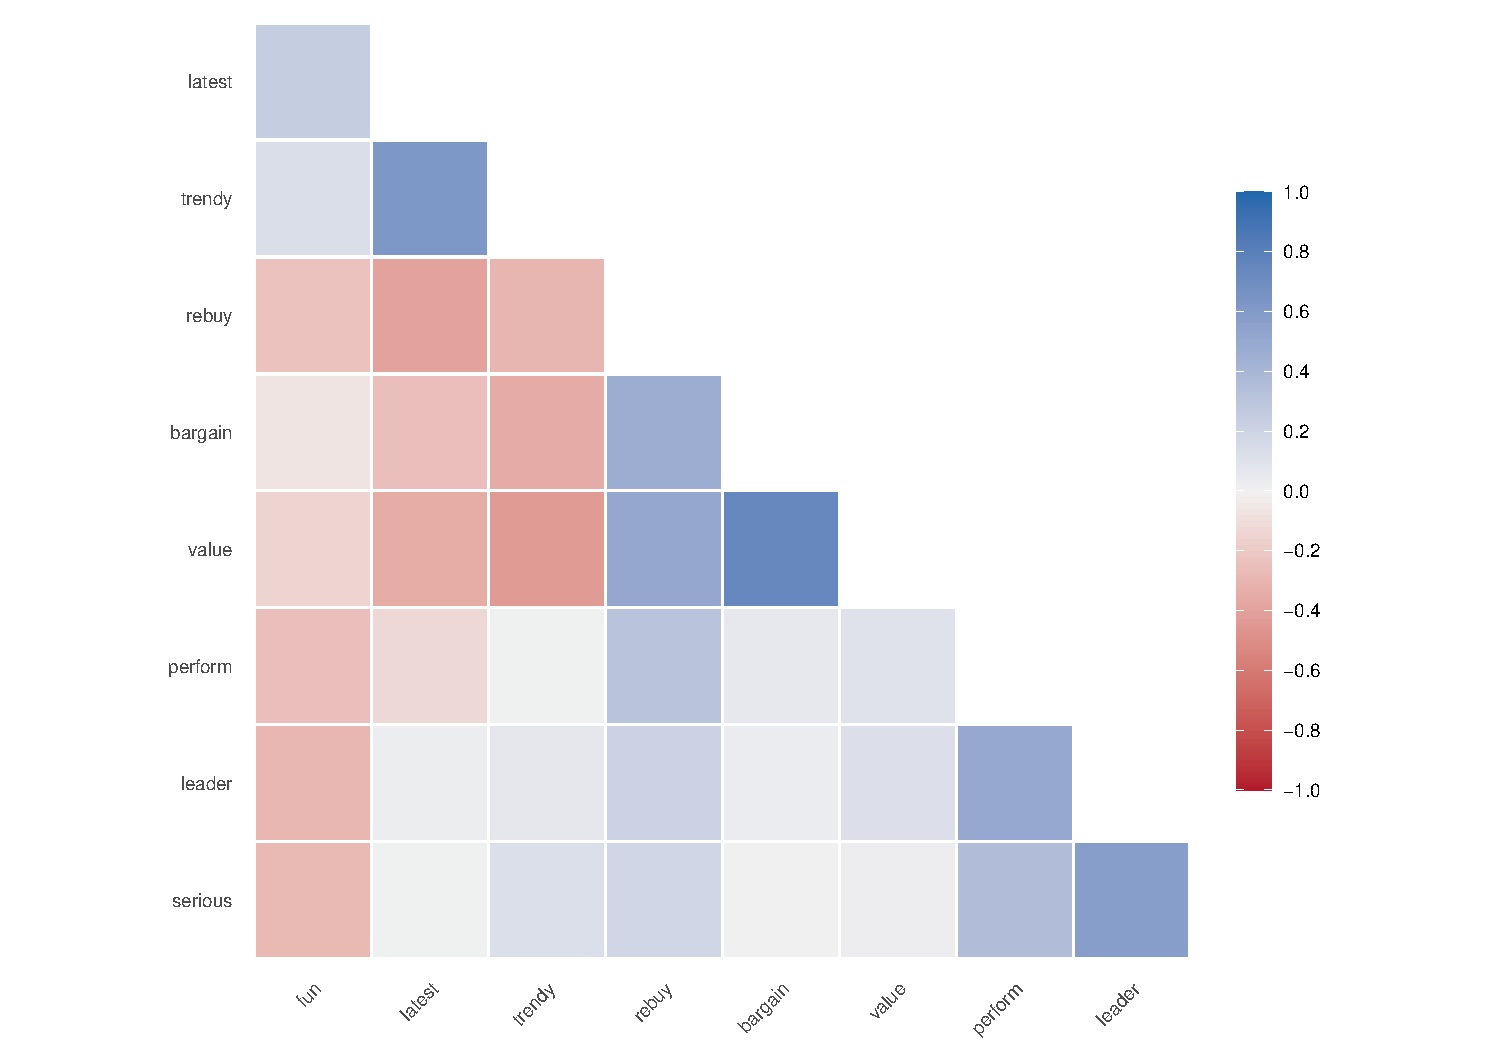
\includegraphics[width=0.5\textwidth,height=\textheight]{008_reducing_data_complexity_files/figure-beamer/unnamed-chunk-6-1.pdf}
\end{center}
\end{frame}

\begin{frame}[fragile]{}
\phantomsection\label{section-8}
\begin{itemize}
\tightlist
\item
  Mean ratings by brand
\end{itemize}

\tiny

\begin{Shaded}
\begin{Highlighting}[]
\NormalTok{brand\_mean }\OtherTok{\textless{}{-}}\NormalTok{ consumer\_brand\_scale }\SpecialCharTok{|\textgreater{}} 
  \FunctionTok{group\_by}\NormalTok{(brand) }\SpecialCharTok{|\textgreater{}} 
  \FunctionTok{summarise}\NormalTok{(}\FunctionTok{across}\NormalTok{(}\FunctionTok{everything}\NormalTok{(), }\AttributeTok{.fns =}\NormalTok{ mean))}
\NormalTok{brand\_mean}
\end{Highlighting}
\end{Shaded}

\begin{verbatim}
# A tibble: 10 x 10
   brand perform leader latest    fun serious bargain   value  trendy   rebuy
   <chr>   <dbl>  <dbl>  <dbl>  <dbl>   <dbl>   <dbl>   <dbl>   <dbl>   <dbl>
 1 a     -0.886  -0.528  0.411  0.657 -0.919   0.214   0.185  -0.525  -0.596 
 2 b      0.931   1.07   0.726 -0.972  1.18    0.0416  0.151   0.740   0.237 
 3 c      0.650   1.16  -0.102 -0.845  1.22   -0.607  -0.441   0.0255 -0.132 
 4 d     -0.680  -0.593  0.352  0.187 -0.692  -0.881  -0.933   0.737  -0.494 
 5 e     -0.564   0.193  0.456  0.296  0.0421  0.552   0.418   0.139   0.0365
 6 f     -0.0587  0.270 -1.26  -0.218  0.589   0.874   1.02   -0.813   1.36  
 7 g      0.918  -0.168 -1.28  -0.517 -0.534   0.897   1.26   -1.28    1.36  
 8 h     -0.0150 -0.298  0.502  0.715 -0.141  -0.738  -0.783   0.864  -0.604 
 9 i      0.335  -0.321  0.356  0.412 -0.149  -0.255  -0.803   0.591  -0.203 
10 j     -0.630  -0.789 -0.154  0.285 -0.602  -0.0971 -0.0738 -0.481  -0.962 
\end{verbatim}
\end{frame}

\begin{frame}[fragile]{}
\phantomsection\label{section-9}
\begin{itemize}
\tightlist
\item
  Mean ratings by brand
\end{itemize}

\tiny

\begin{Shaded}
\begin{Highlighting}[]
\NormalTok{brand\_mean\_longer }\OtherTok{\textless{}{-}}\NormalTok{ brand\_mean }\SpecialCharTok{|\textgreater{}} 
  \FunctionTok{pivot\_longer}\NormalTok{(}\AttributeTok{cols =}\NormalTok{ perform}\SpecialCharTok{:}\NormalTok{rebuy,}
               \AttributeTok{names\_to =} \StringTok{"perceptual\_adjectives"}\NormalTok{,}
               \AttributeTok{values\_to =} \StringTok{"value\_mean"}\NormalTok{) }\SpecialCharTok{|\textgreater{}} 
  \FunctionTok{mutate}\NormalTok{(}\AttributeTok{brand =} \FunctionTok{fct\_reorder}\NormalTok{(}\AttributeTok{.f =}\NormalTok{ brand, }\AttributeTok{.x =}\NormalTok{ value\_mean),}
         \AttributeTok{perceptual\_adjectives =} \FunctionTok{fct\_reorder}\NormalTok{(}\AttributeTok{.f =}\NormalTok{ perceptual\_adjectives, }\AttributeTok{.x =}\NormalTok{ value\_mean))}
\NormalTok{brand\_mean\_longer}
\end{Highlighting}
\end{Shaded}

\begin{verbatim}
# A tibble: 90 x 3
   brand perceptual_adjectives value_mean
   <fct> <fct>                      <dbl>
 1 a     perform                   -0.886
 2 a     leader                    -0.528
 3 a     latest                     0.411
 4 a     fun                        0.657
 5 a     serious                   -0.919
 6 a     bargain                    0.214
 7 a     value                      0.185
 8 a     trendy                    -0.525
 9 a     rebuy                     -0.596
10 b     perform                    0.931
# i 80 more rows
\end{verbatim}
\end{frame}

\begin{frame}[fragile]{}
\phantomsection\label{section-10}
\begin{itemize}
\tightlist
\item
  Heat map mean ratings by brand
\end{itemize}

\tiny

\begin{Shaded}
\begin{Highlighting}[]
\FunctionTok{library}\NormalTok{(tidyheatmaps)}
\FunctionTok{tidyheatmap}\NormalTok{(}\AttributeTok{df =}\NormalTok{ brand\_mean\_longer, }
            \AttributeTok{rows =}\NormalTok{ brand, }\AttributeTok{columns =}\NormalTok{ perceptual\_adjectives, }\AttributeTok{values =}\NormalTok{ value\_mean,}
            \AttributeTok{cluster\_rows =} \ConstantTok{TRUE}\NormalTok{, }\AttributeTok{cluster\_cols =} \ConstantTok{TRUE}\NormalTok{,}
            \AttributeTok{clustering\_method =} \StringTok{"complete"}\NormalTok{, }\CommentTok{\# See ?hclust and chapter 11}
            \AttributeTok{display\_numbers =} \ConstantTok{TRUE}\NormalTok{, }\AttributeTok{border\_color =} \StringTok{"black"}\NormalTok{, }\AttributeTok{fontsize =} \DecValTok{12}\NormalTok{)}
\end{Highlighting}
\end{Shaded}

\begin{center}
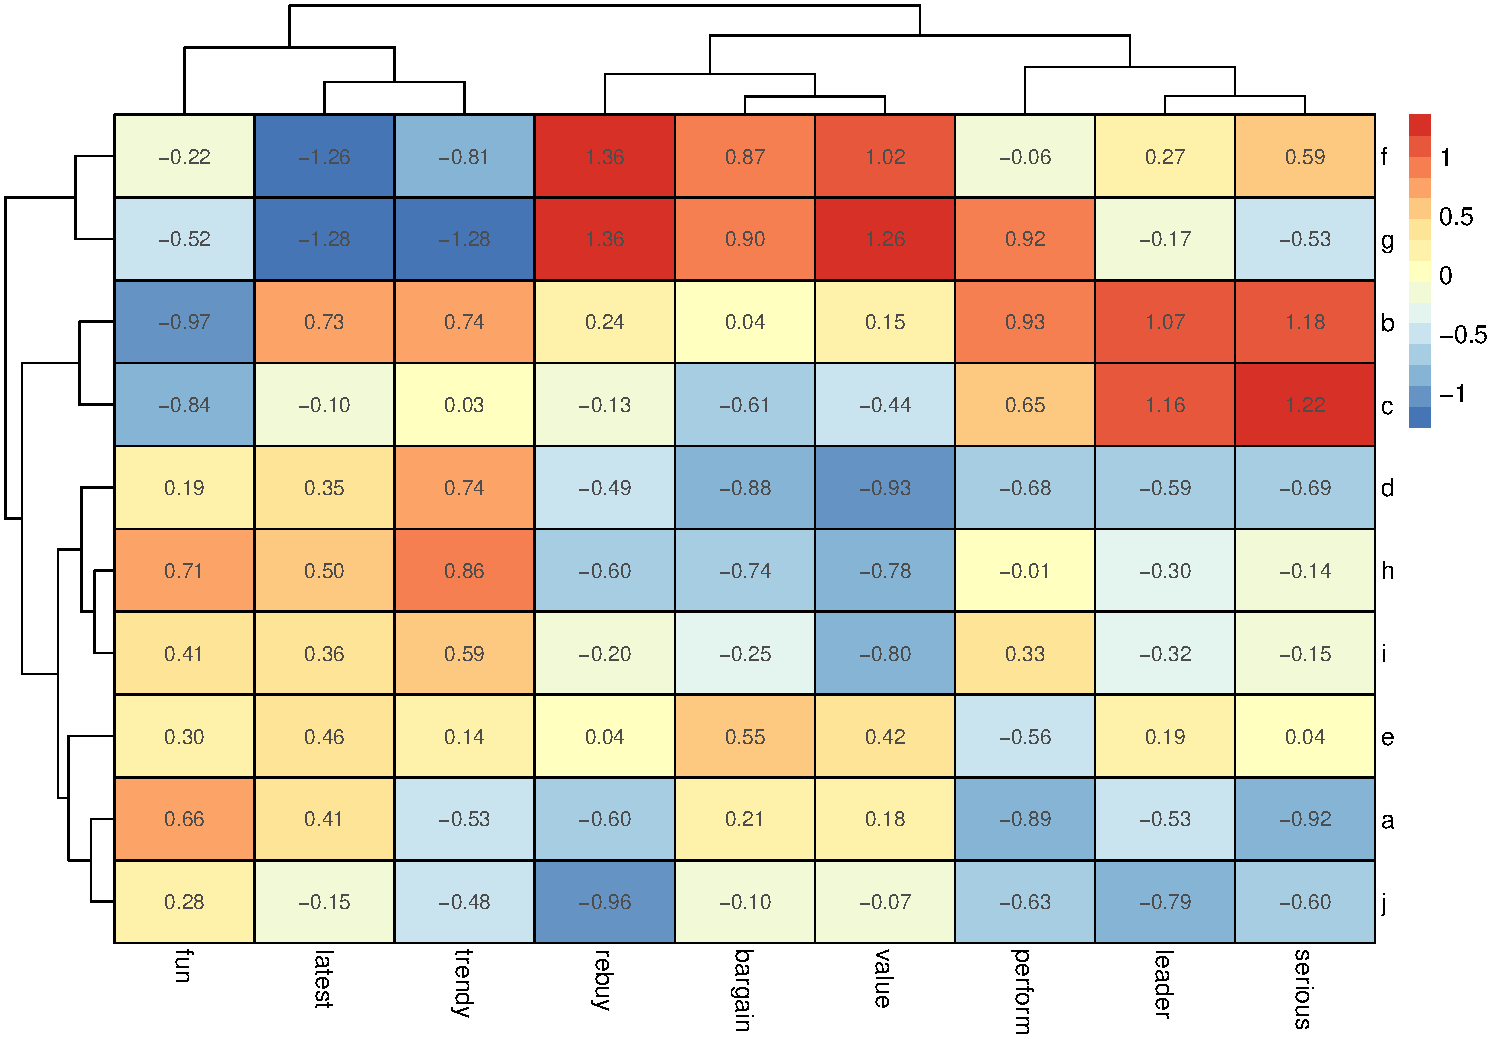
\includegraphics[width=0.5\textwidth,height=\textheight]{008_reducing_data_complexity_files/figure-beamer/unnamed-chunk-9-1.pdf}
\end{center}
\end{frame}

\begin{frame}[fragile]{}
\phantomsection\label{section-11}
\begin{itemize}
\item
  Principal component analysis (PCA) and perceptual maps

  \begin{itemize}
  \tightlist
  \item
    PCA reduced example
  \end{itemize}
\end{itemize}

\tiny

\begin{Shaded}
\begin{Highlighting}[]
\FunctionTok{set.seed}\NormalTok{(}\AttributeTok{seed =} \DecValTok{1234}\NormalTok{)}
\NormalTok{consumer\_brand\_sample }\OtherTok{\textless{}{-}}\NormalTok{ consumer\_brand }\SpecialCharTok{|\textgreater{}}
  \FunctionTok{slice\_sample}\NormalTok{(}\AttributeTok{n =} \DecValTok{1}\NormalTok{, }\AttributeTok{by =}\NormalTok{ brand) }\SpecialCharTok{|\textgreater{}} 
  \FunctionTok{select}\NormalTok{(brand, perform, leader)}
\NormalTok{consumer\_brand\_sample}
\end{Highlighting}
\end{Shaded}

\begin{verbatim}
# A tibble: 10 x 3
   brand perform leader
   <chr>   <dbl>  <dbl>
 1 a           2      4
 2 b           9      6
 3 c           5      6
 4 d           3      3
 5 e           1      5
 6 f           8      6
 7 g          10      7
 8 h           8      1
 9 i           8      2
10 j           4      1
\end{verbatim}
\end{frame}

\begin{frame}{}
\phantomsection\label{section-12}
\begin{itemize}
\item
  Principal component analysis (PCA) and perceptual maps

  \begin{itemize}
  \tightlist
  \item
    Visualizing original data
  \end{itemize}
\end{itemize}

\begin{center}
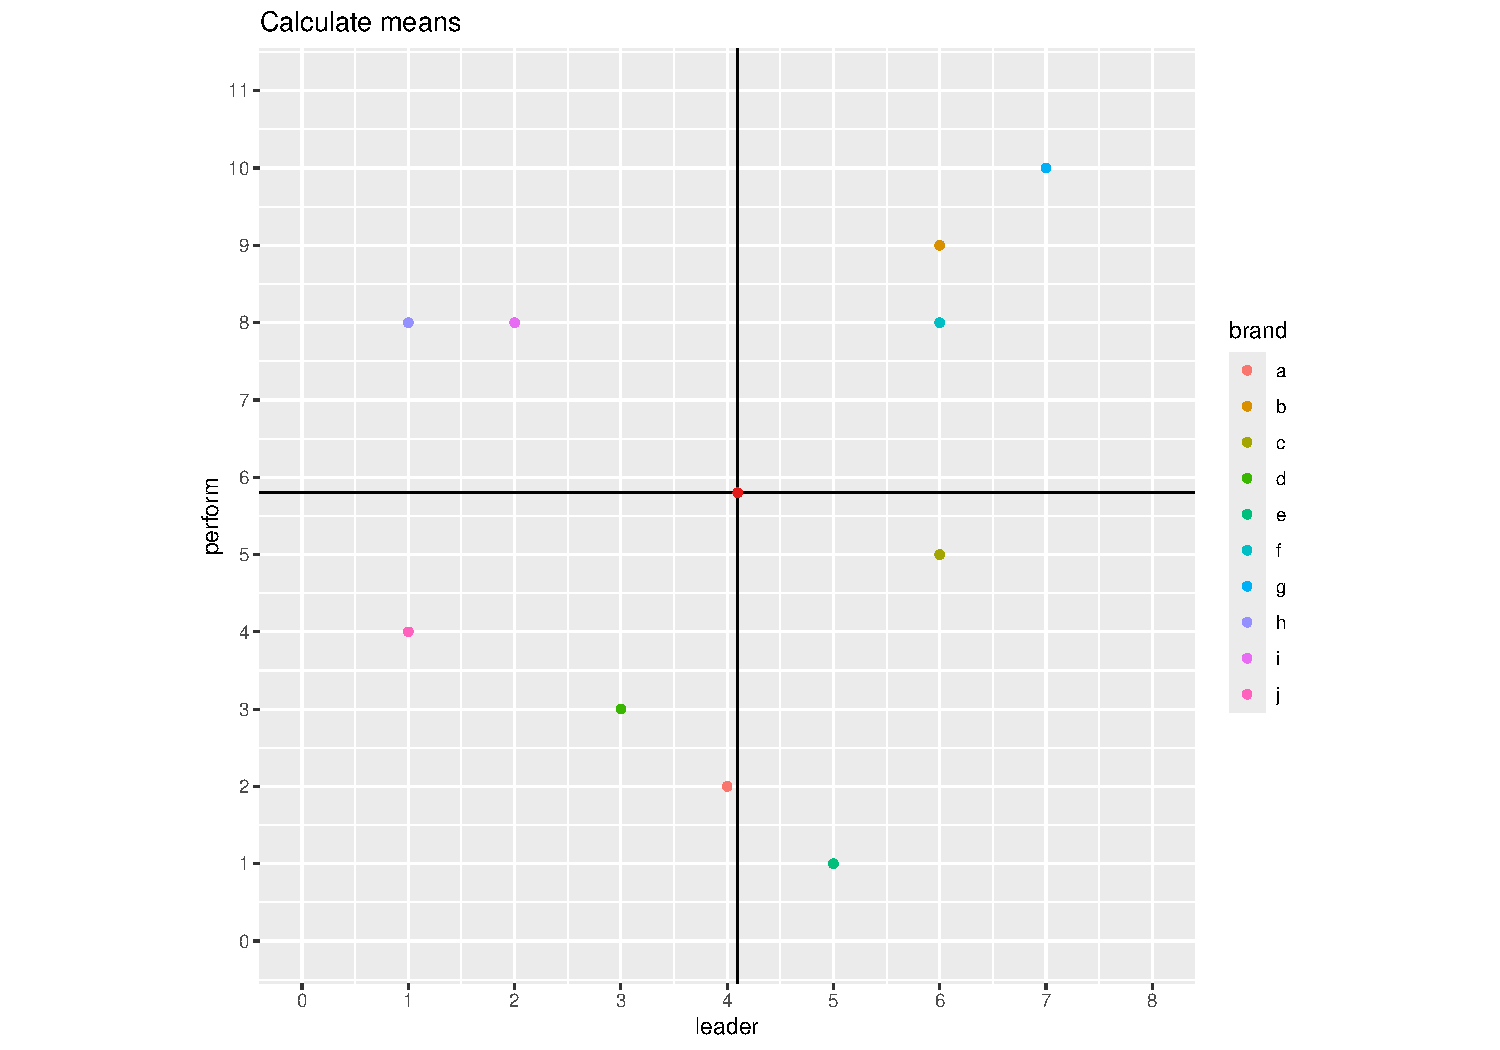
\includegraphics[width=0.7\textwidth,height=\textheight]{008_reducing_data_complexity_files/figure-beamer/unnamed-chunk-11-1.pdf}
\end{center}
\end{frame}

\begin{frame}{}
\phantomsection\label{section-13}
\begin{itemize}
\item
  Principal component analysis (PCA) and perceptual maps

  \begin{itemize}
  \tightlist
  \item
    Centering data using the mean
  \end{itemize}
\end{itemize}

\begin{center}
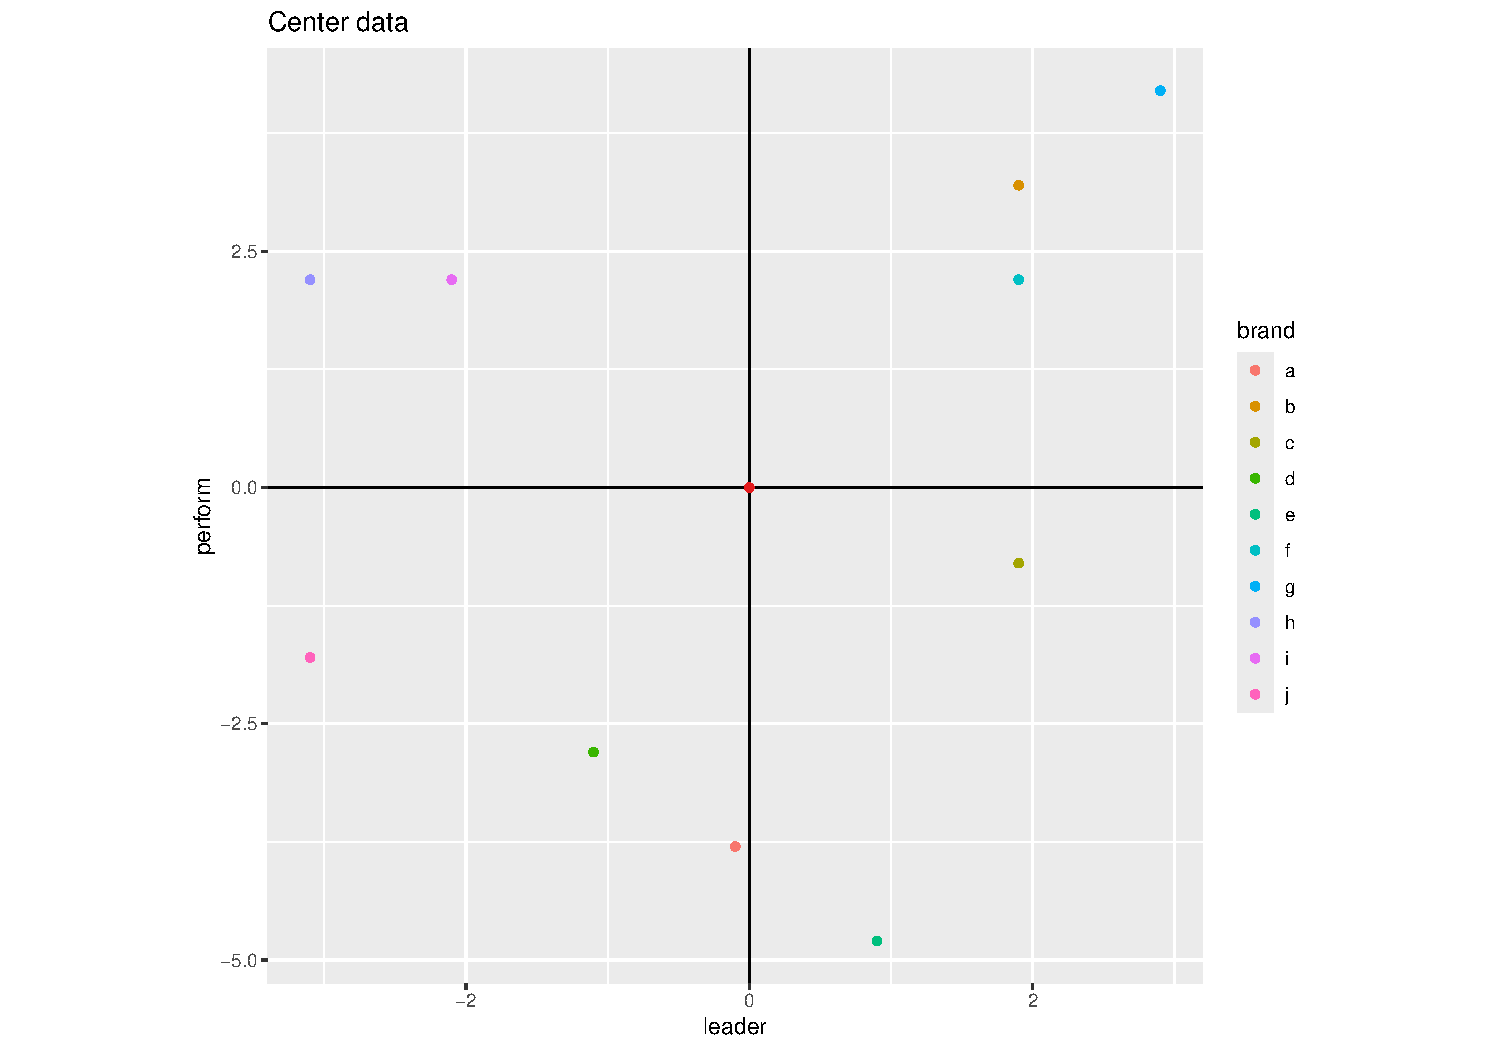
\includegraphics[width=0.7\textwidth,height=\textheight]{008_reducing_data_complexity_files/figure-beamer/unnamed-chunk-12-1.pdf}
\end{center}
\end{frame}

\begin{frame}{}
\phantomsection\label{section-14}
\begin{itemize}
\item
  Principal component analysis (PCA) and perceptual maps

  \begin{itemize}
  \tightlist
  \item
    Scaling data using the standard deviation
  \end{itemize}
\end{itemize}

\begin{center}
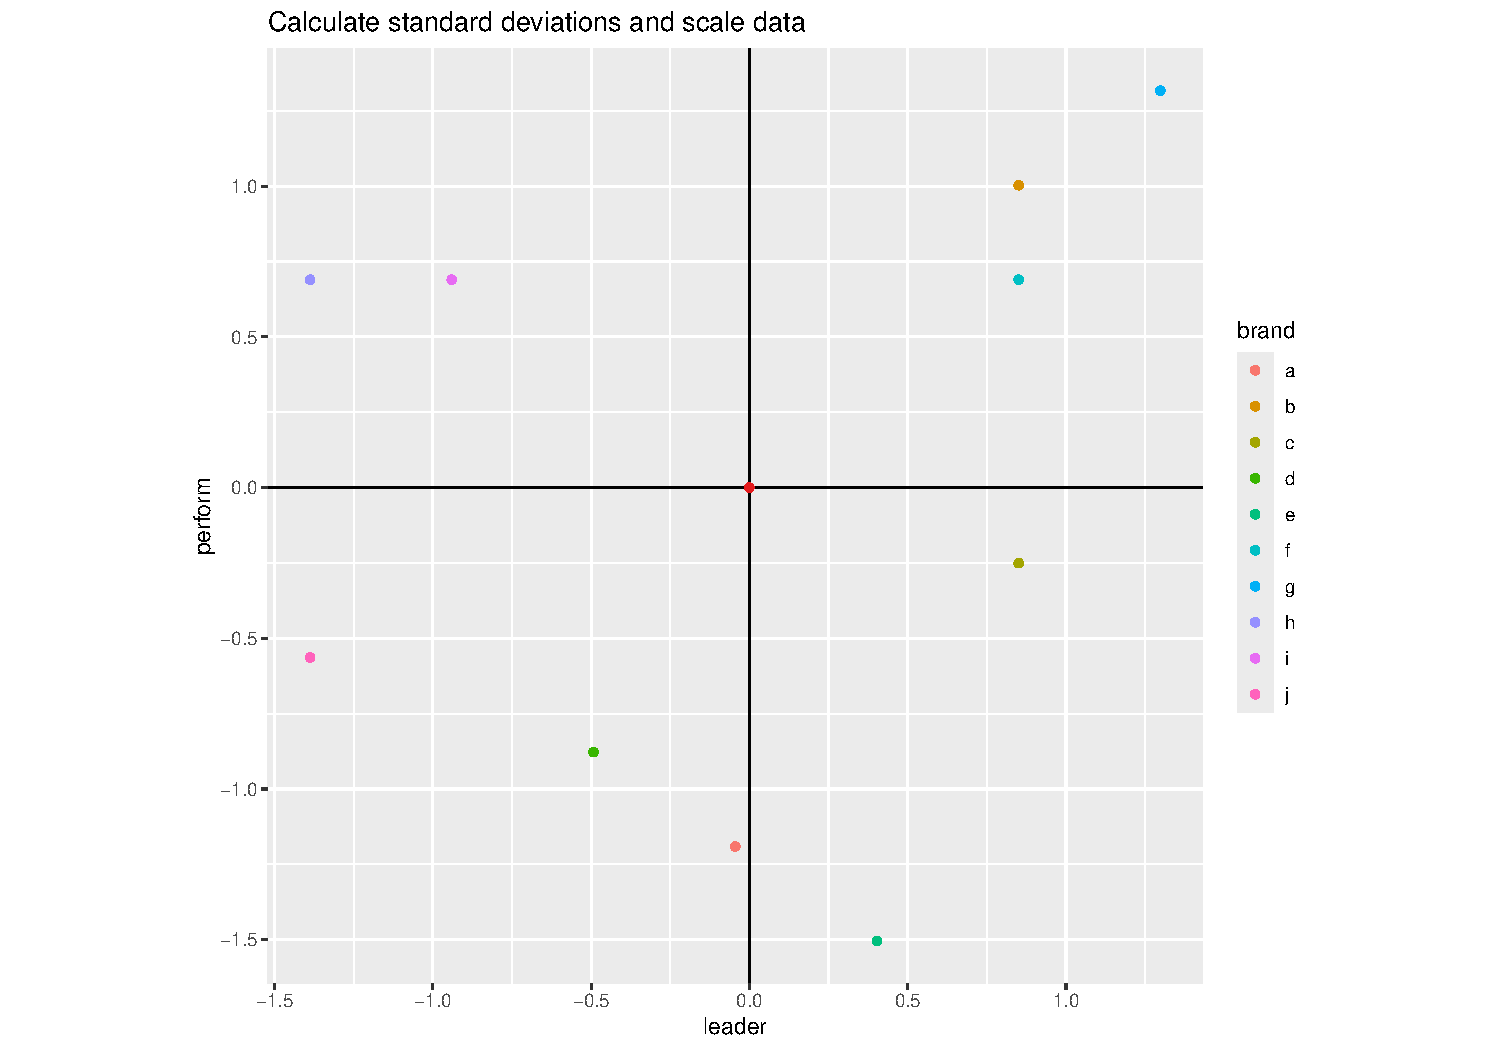
\includegraphics[width=0.7\textwidth,height=\textheight]{008_reducing_data_complexity_files/figure-beamer/unnamed-chunk-13-1.pdf}
\end{center}
\end{frame}

\begin{frame}{}
\phantomsection\label{section-15}
\begin{itemize}
\item
  Principal component analysis (PCA) and perceptual maps

  \begin{itemize}
  \tightlist
  \item
    Fitting a line by performing an orthogonal regression
  \end{itemize}
\end{itemize}

\begin{center}
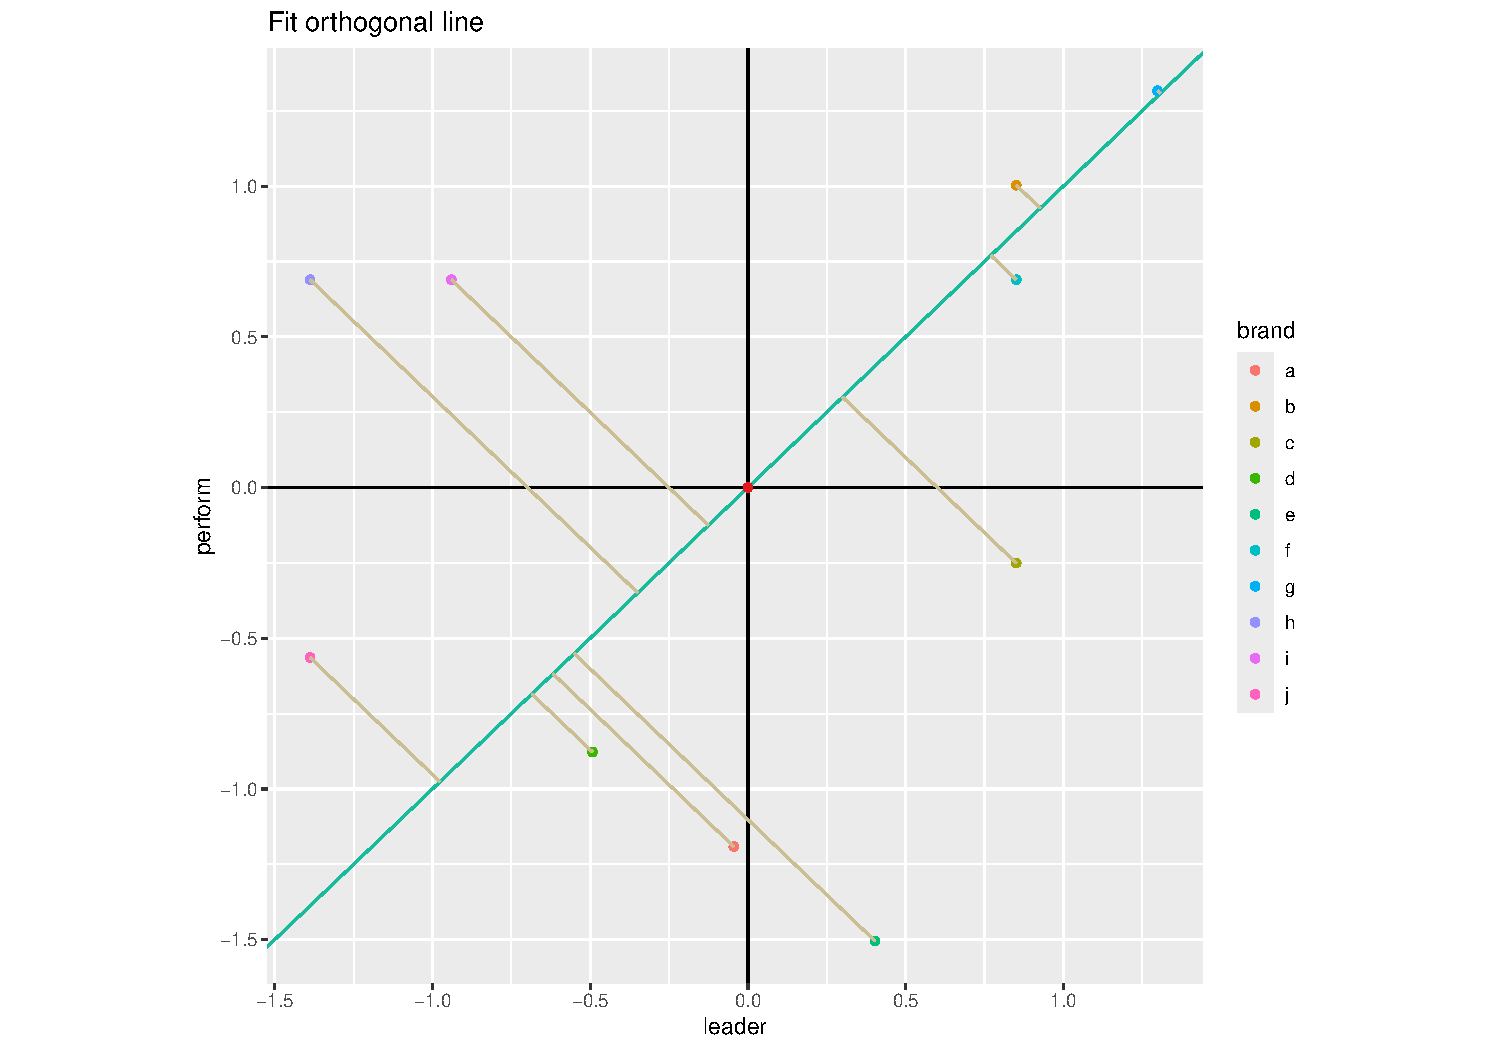
\includegraphics[width=0.7\textwidth,height=\textheight]{008_reducing_data_complexity_files/figure-beamer/unnamed-chunk-14-1.pdf}
\end{center}
\end{frame}

\begin{frame}{}
\phantomsection\label{section-16}
\begin{itemize}
\item
  Principal component analysis (PCA) and perceptual maps

  \begin{itemize}
  \tightlist
  \item
    Find a line orthogonal to the fitted line
  \end{itemize}
\end{itemize}

\begin{center}
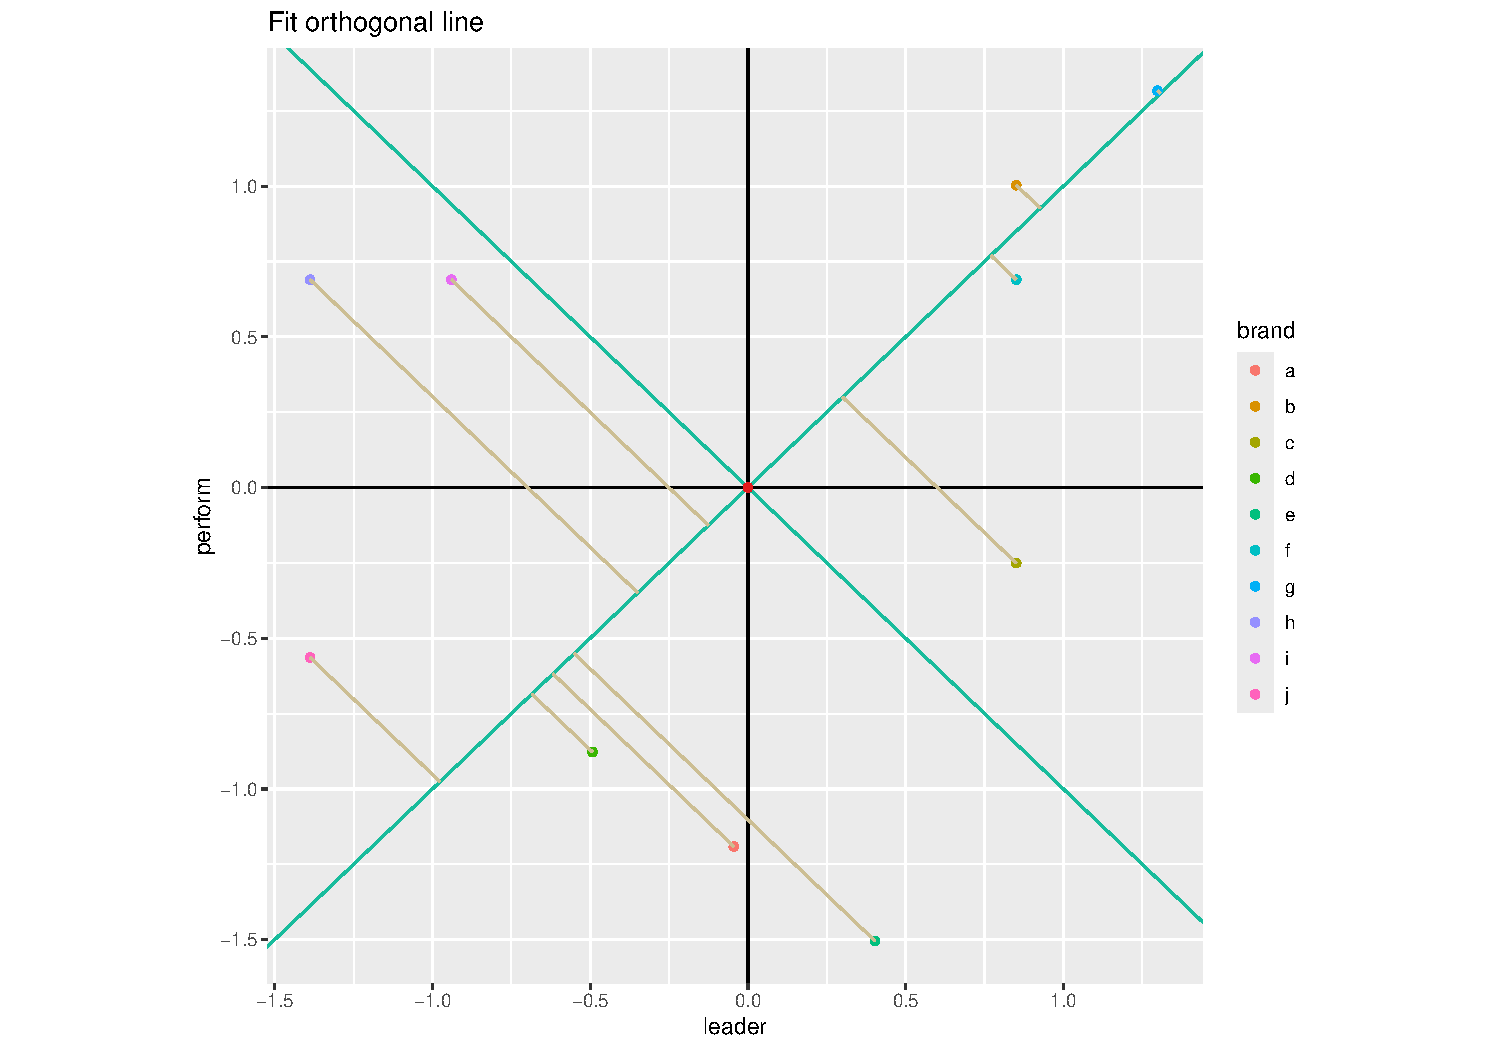
\includegraphics[width=0.7\textwidth,height=\textheight]{008_reducing_data_complexity_files/figure-beamer/unnamed-chunk-15-1.pdf}
\end{center}
\end{frame}

\begin{frame}{}
\phantomsection\label{section-17}
\begin{itemize}
\item
  Principal component analysis (PCA) and perceptual maps

  \begin{itemize}
  \tightlist
  \item
    Find the orthogonal distances between the points and the new line
  \end{itemize}
\end{itemize}

\begin{center}
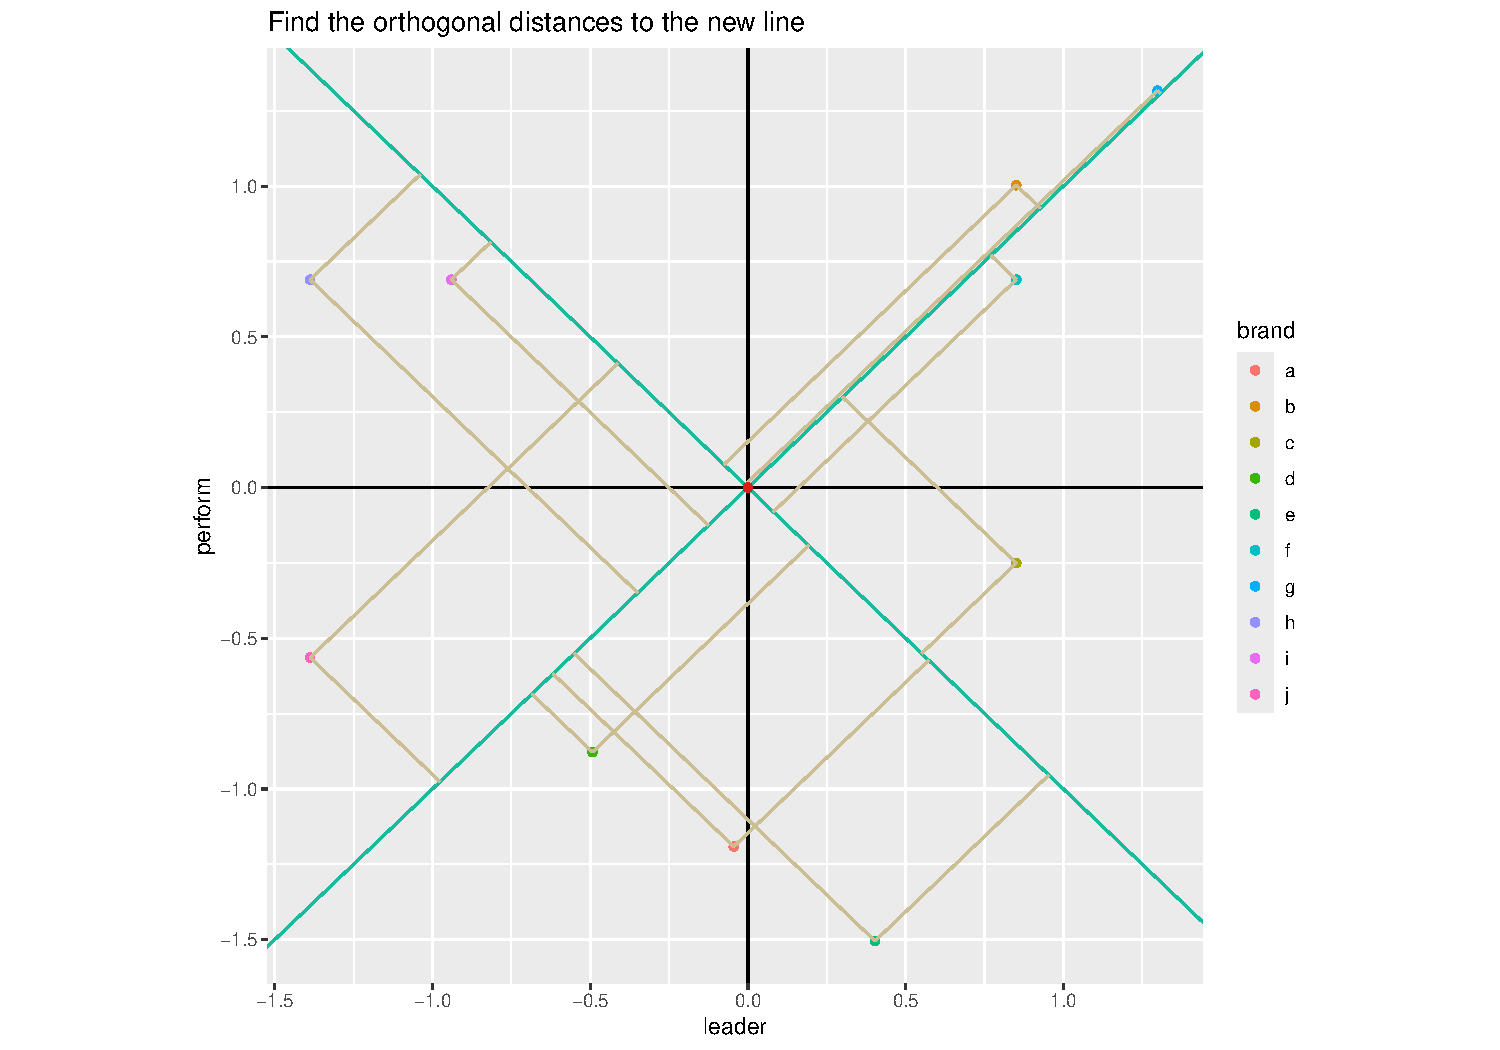
\includegraphics[width=0.7\textwidth,height=\textheight]{008_reducing_data_complexity_files/figure-beamer/unnamed-chunk-16-1.pdf}
\end{center}
\end{frame}

\begin{frame}{}
\phantomsection\label{section-18}
\begin{itemize}
\item
  Principal component analysis (PCA) and perceptual maps

  \begin{itemize}
  \tightlist
  \item
    Project the points onto each line
  \end{itemize}
\end{itemize}

\begin{center}
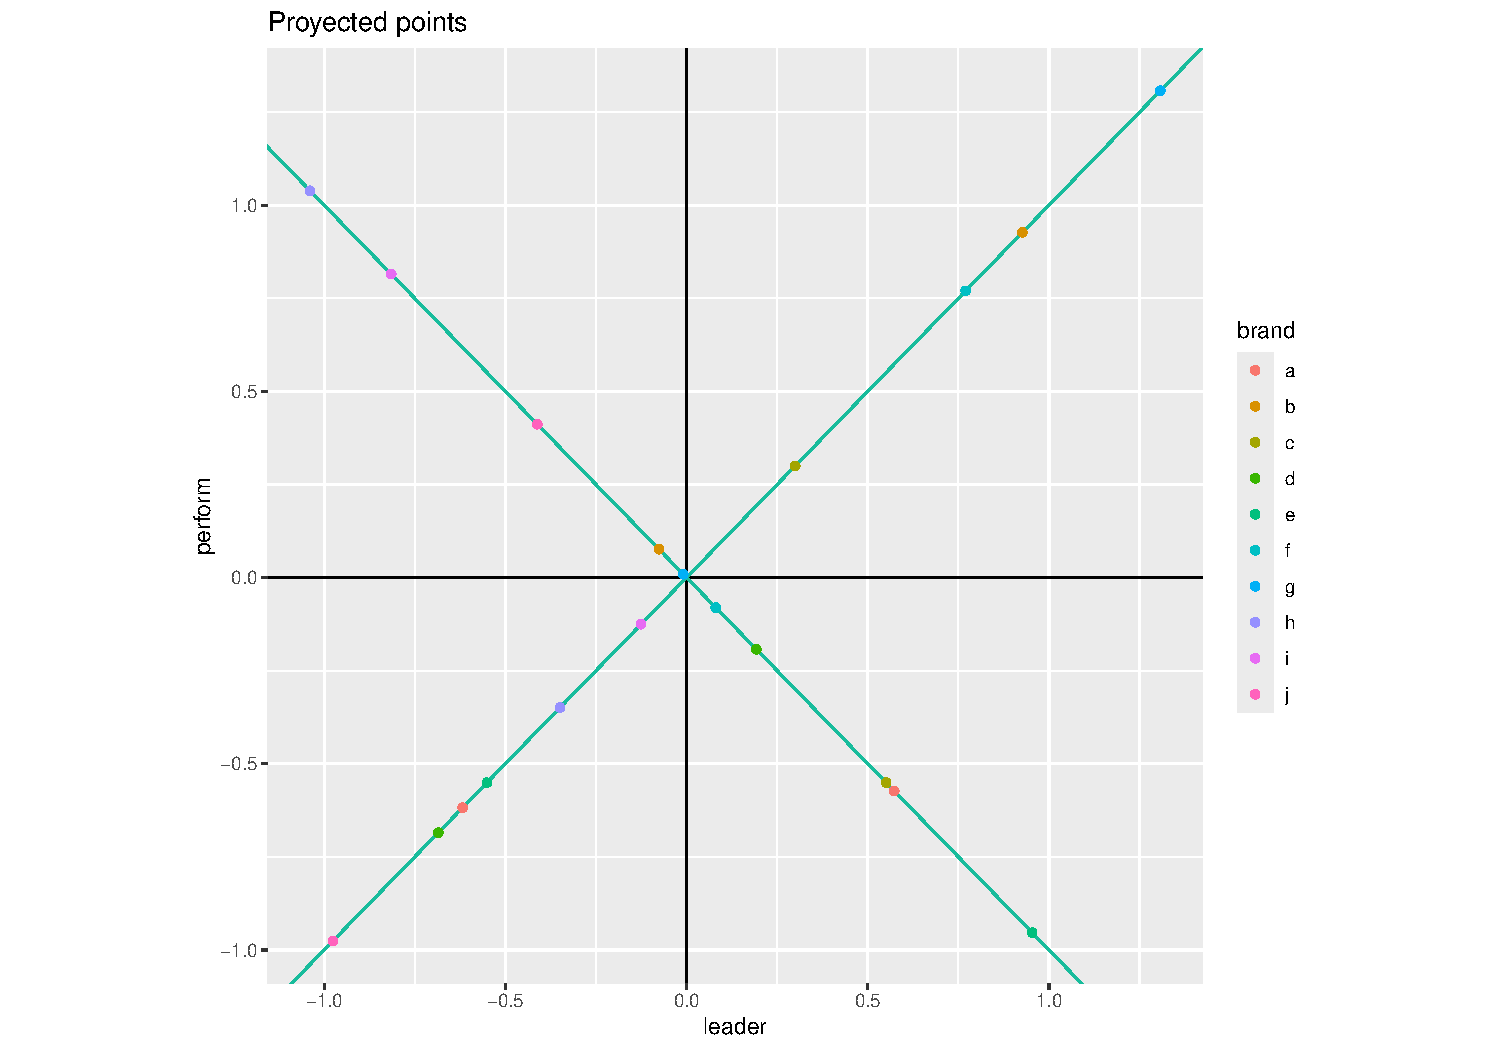
\includegraphics[width=0.7\textwidth,height=\textheight]{008_reducing_data_complexity_files/figure-beamer/unnamed-chunk-17-1.pdf}
\end{center}
\end{frame}

\begin{frame}{}
\phantomsection\label{section-19}
\begin{itemize}
\item
  Principal component analysis (PCA) and perceptual maps

  \begin{itemize}
  \tightlist
  \item
    Rotate the fitted line and the projected points around \((0,0)\)
  \end{itemize}
\end{itemize}

\begin{center}
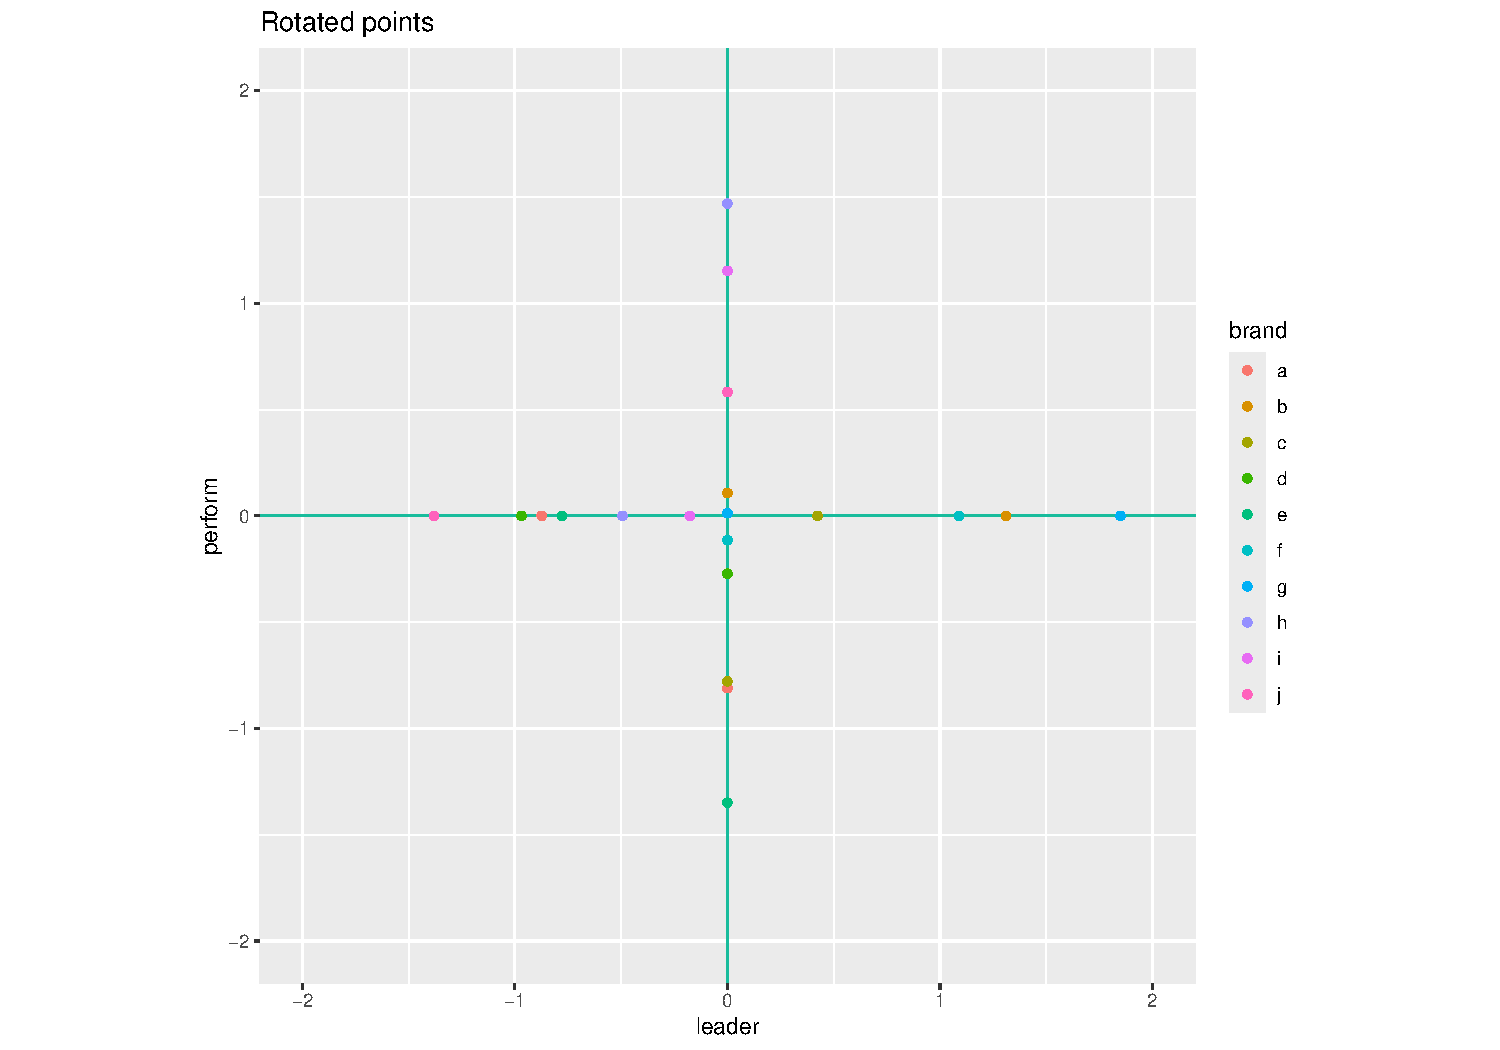
\includegraphics[width=0.7\textwidth,height=\textheight]{008_reducing_data_complexity_files/figure-beamer/unnamed-chunk-18-1.pdf}
\end{center}
\end{frame}

\begin{frame}{}
\phantomsection\label{section-20}
\begin{itemize}
\item
  Principal component analysis (PCA) and perceptual maps

  \begin{itemize}
  \tightlist
  \item
    Fix the new points based on the projected points
  \end{itemize}
\end{itemize}

\begin{center}
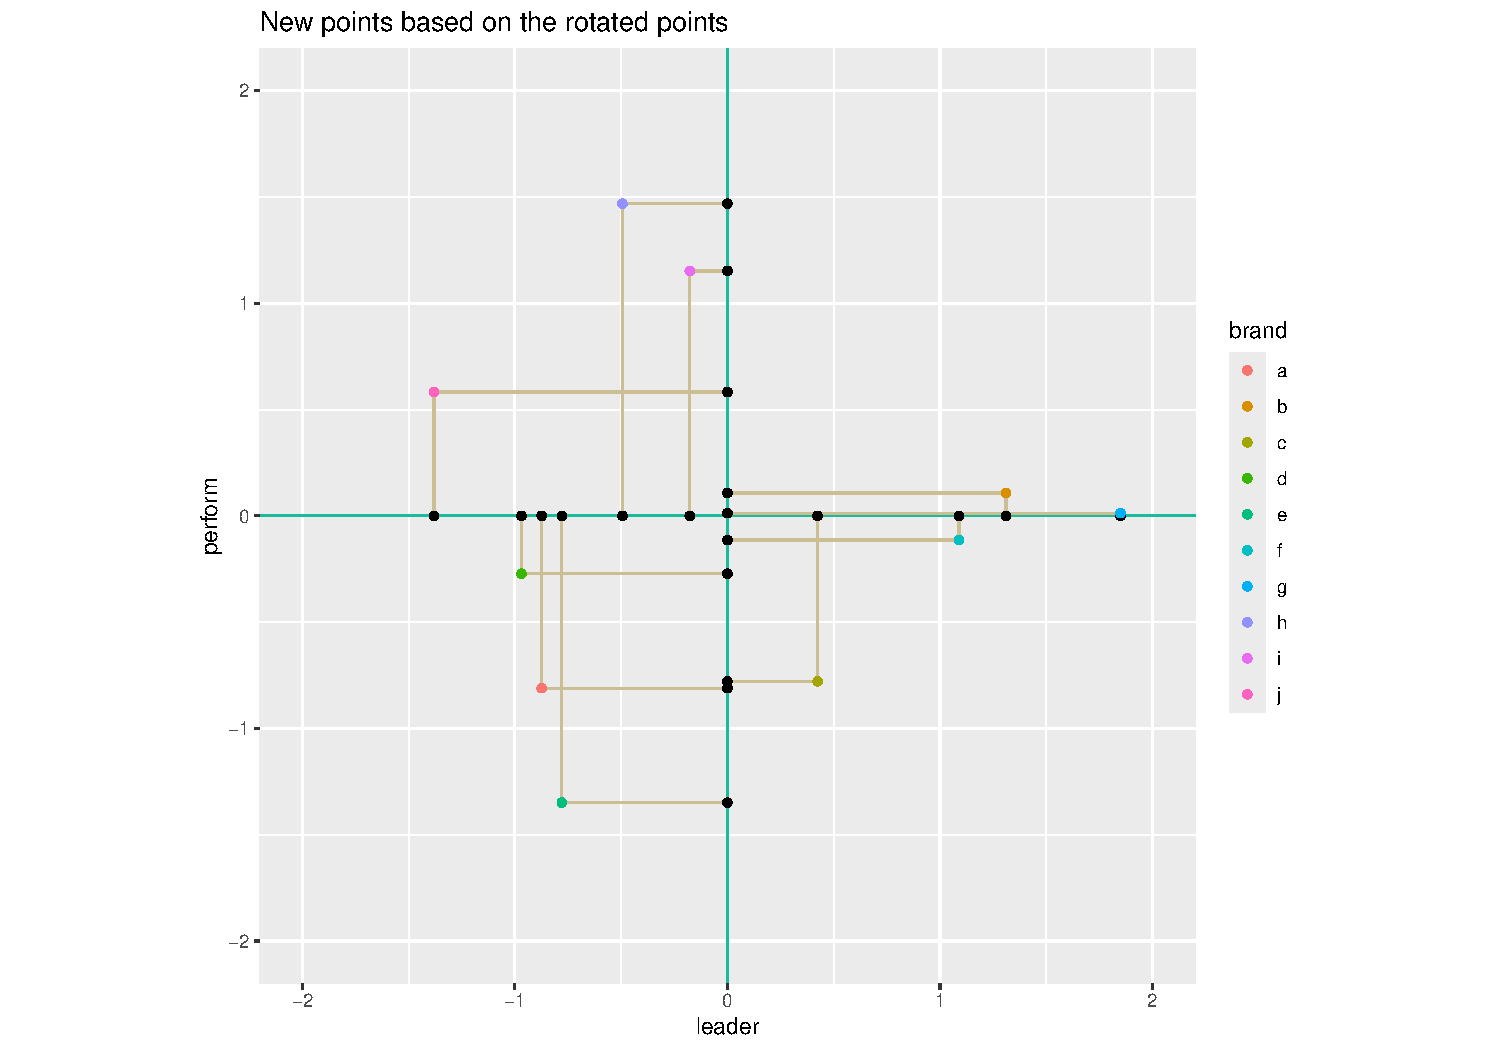
\includegraphics[width=0.7\textwidth,height=\textheight]{008_reducing_data_complexity_files/figure-beamer/unnamed-chunk-19-1.pdf}
\end{center}
\end{frame}

\begin{frame}{}
\phantomsection\label{section-21}
\begin{itemize}
\item
  Principal component analysis (PCA) and perceptual maps

  \begin{itemize}
  \tightlist
  \item
    Apply data complexity reduction by focusing on the horizontal axis
  \end{itemize}
\end{itemize}

\begin{center}
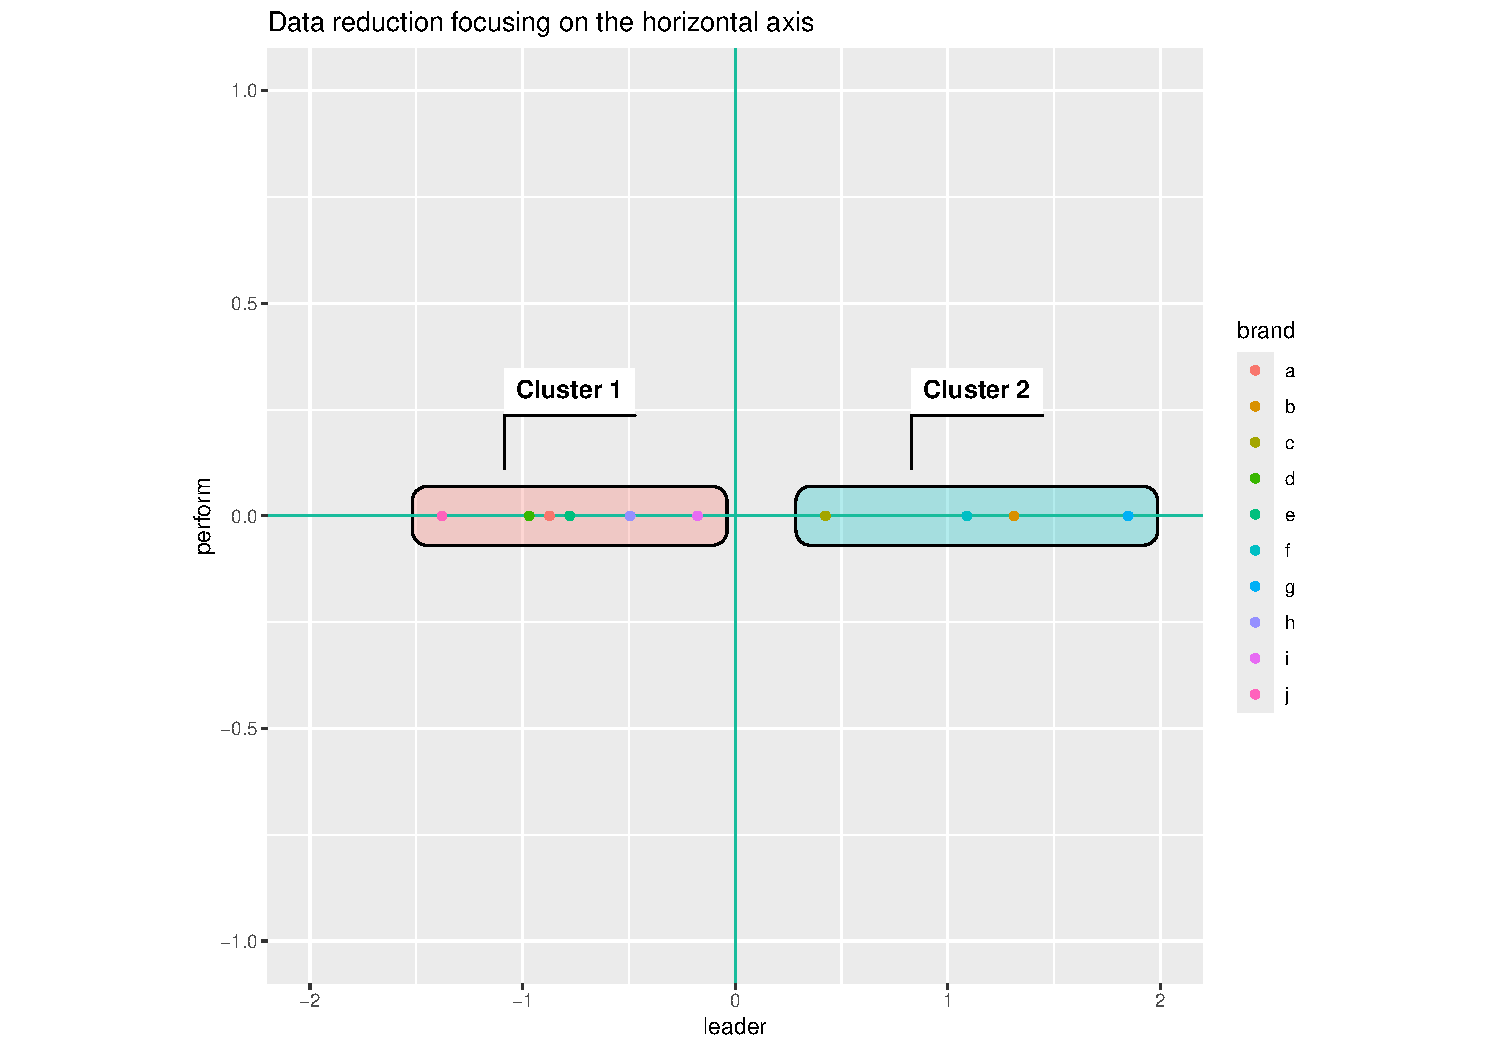
\includegraphics[width=0.7\textwidth,height=\textheight]{008_reducing_data_complexity_files/figure-beamer/unnamed-chunk-20-1.pdf}
\end{center}
\end{frame}

\begin{frame}{}
\phantomsection\label{section-22}
\begin{itemize}
\item
  Principal component analysis (PCA) and perceptual maps

  \begin{itemize}
  \tightlist
  \item
    Recover the data that was reduced when focusing in the horizontal
    axis
  \end{itemize}
\end{itemize}

\begin{center}
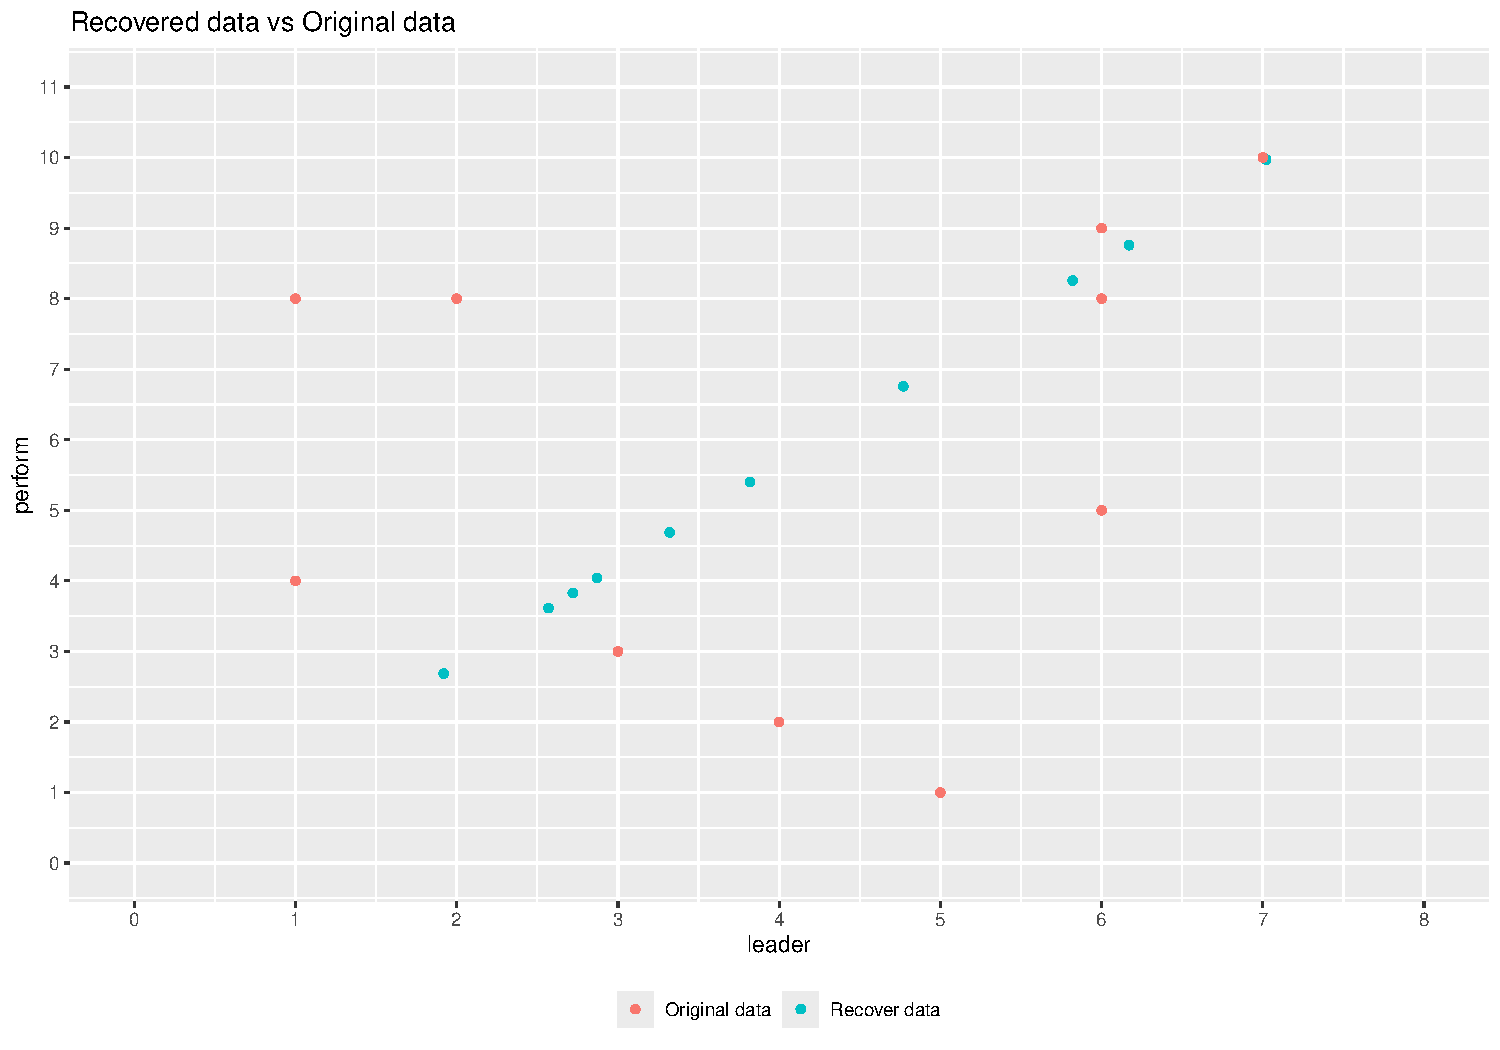
\includegraphics[width=0.7\textwidth,height=\textheight]{008_reducing_data_complexity_files/figure-beamer/unnamed-chunk-21-1.pdf}
\end{center}
\end{frame}

\section{Understanding the reduction of data
complexity}\label{understanding-the-reduction-of-data-complexity}

\begin{frame}{}
\phantomsection\label{section-23}
\begin{figure}[H]

{\centering 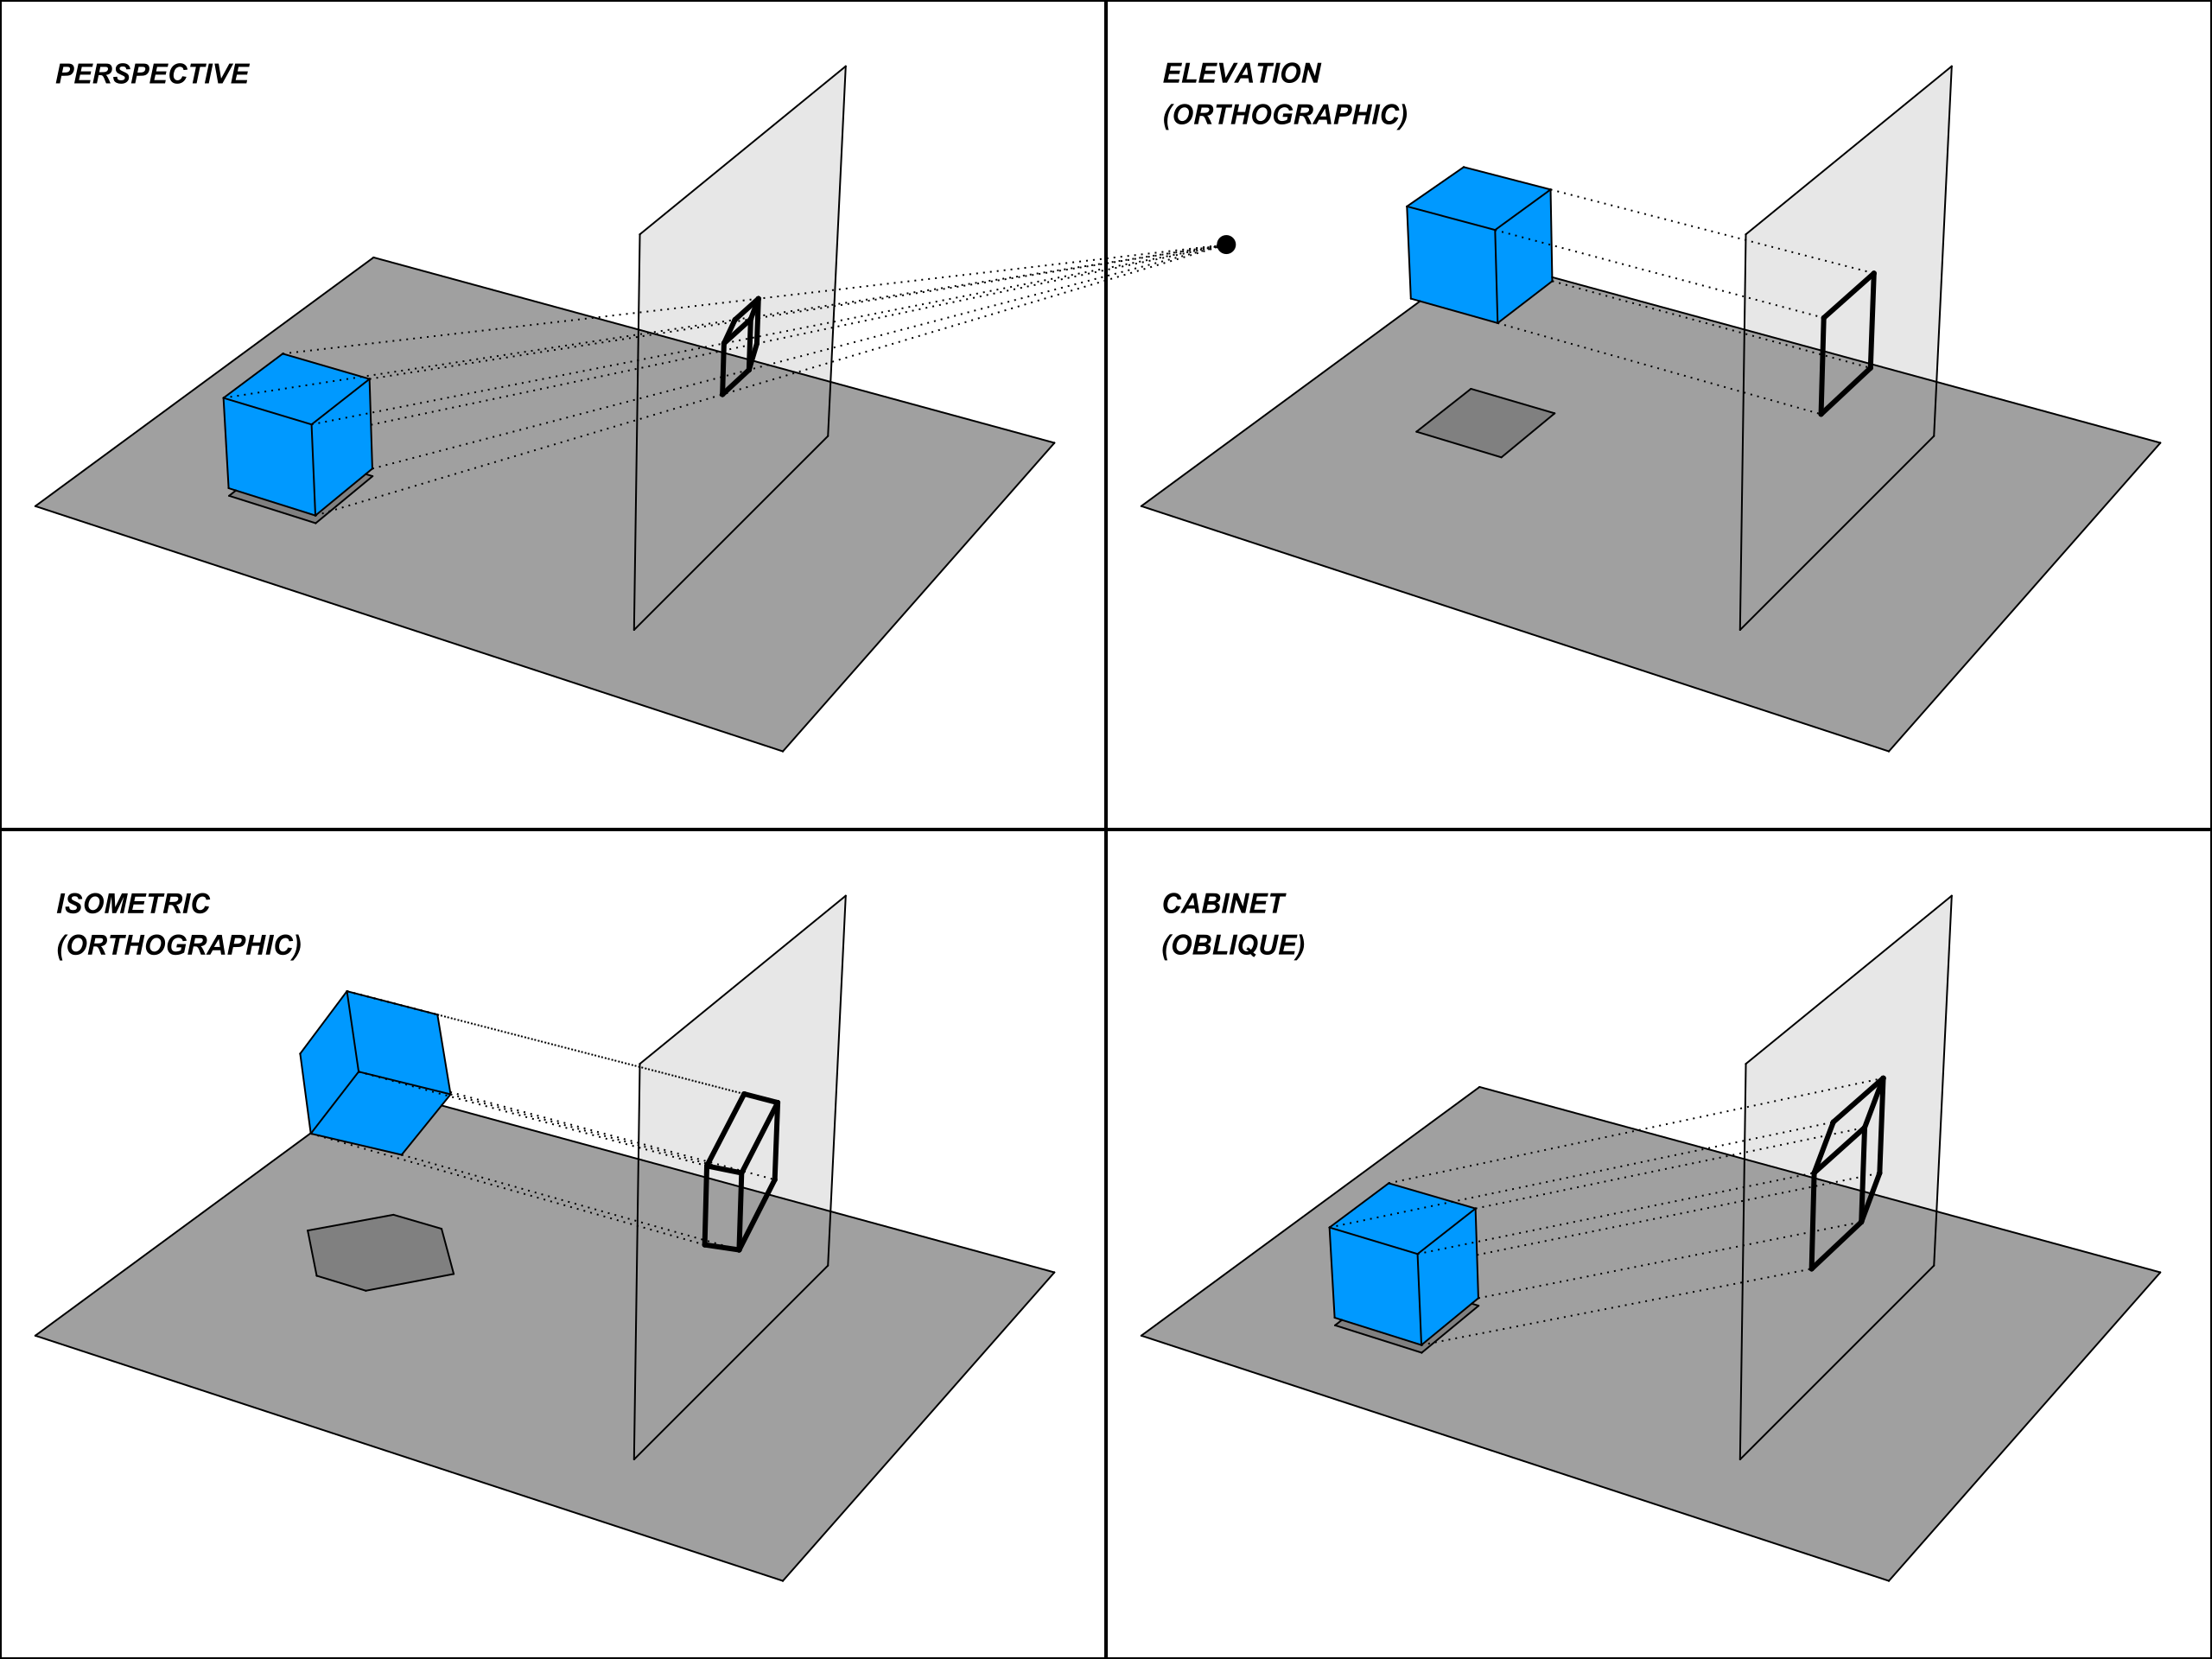
\includegraphics[width=3.125in,height=3.125in]{../000_images/008_various_projections_of_cube_above_plane.png}

}

\caption{Various projections of cube above plane by Michael Horvath (aka
Datumizer) 2021-05-10}

\end{figure}%
\end{frame}

\begin{frame}{}
\phantomsection\label{section-24}
\begin{itemize}
\item
  Principal component analysis (PCA) and perceptual maps

  \begin{itemize}
  \tightlist
  \item
    Using an image to understand data complexity reduction
  \end{itemize}
\end{itemize}

\begin{center}
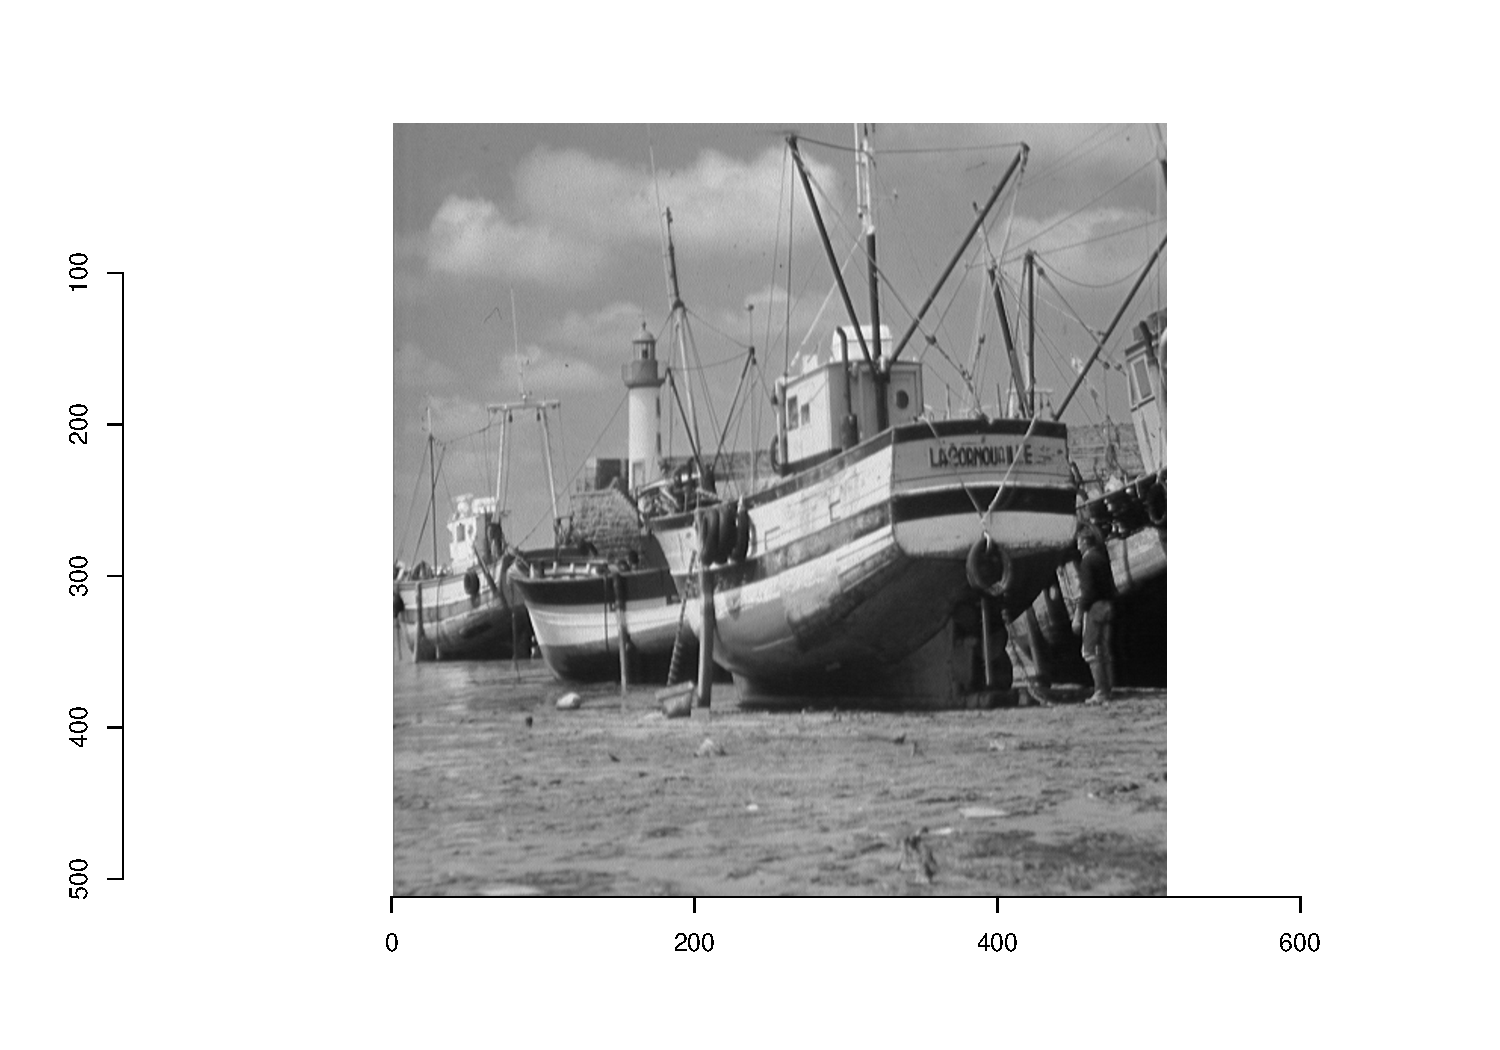
\includegraphics[width=0.7\textwidth,height=\textheight]{008_reducing_data_complexity_files/figure-beamer/unnamed-chunk-22-1.pdf}
\end{center}
\end{frame}

\begin{frame}[fragile]{}
\phantomsection\label{section-25}
\begin{itemize}
\item
  Principal component analysis (PCA) and perceptual maps

  \begin{itemize}
  \item
    Represent and image as data

    \begin{itemize}
    \tightlist
    \item
      \texttt{x,y}: position of a point in a cartesian plane \((x,y)\)
    \item
      \texttt{value}: a gray scale where \(0\) is white, \(1\) is black
      and \((0,1)\) is an intermediate color between white and black
    \end{itemize}
  \end{itemize}
\end{itemize}

\tiny

\begin{verbatim}
# A tibble: 262,144 x 3
       x     y value
   <int> <int> <dbl>
 1     1     1 0.498
 2     2     1 0.482
 3     3     1 0.490
 4     4     1 0.471
 5     5     1 0.494
 6     6     1 0.482
 7     7     1 0.498
 8     8     1 0.502
 9     9     1 0.490
10    10     1 0.506
# i 262,134 more rows
\end{verbatim}
\end{frame}

\begin{frame}[fragile]{}
\phantomsection\label{section-26}
\begin{itemize}
\item
  Principal component analysis (PCA) and perceptual maps

  \begin{itemize}
  \tightlist
  \item
    Prepare data for PCA
  \end{itemize}
\end{itemize}

\tiny

\begin{verbatim}
# A tibble: 512 x 513
       x   `1`   `2`   `3`   `4`   `5`   `6`   `7`   `8`   `9`  `10`  `11`  `12`
   <int> <dbl> <dbl> <dbl> <dbl> <dbl> <dbl> <dbl> <dbl> <dbl> <dbl> <dbl> <dbl>
 1     1 0.498 0.502 0.502 0.486 0.494 0.490 0.498 0.482 0.494 0.486 0.478 0.494
 2     2 0.482 0.494 0.486 0.498 0.490 0.498 0.498 0.529 0.502 0.502 0.494 0.498
 3     3 0.490 0.502 0.502 0.502 0.502 0.494 0.494 0.471 0.486 0.498 0.502 0.490
 4     4 0.471 0.478 0.494 0.506 0.494 0.494 0.486 0.502 0.502 0.486 0.494 0.478
 5     5 0.494 0.490 0.498 0.475 0.494 0.502 0.471 0.475 0.490 0.498 0.482 0.490
 6     6 0.482 0.490 0.471 0.502 0.490 0.502 0.498 0.482 0.482 0.475 0.498 0.475
 7     7 0.498 0.478 0.502 0.506 0.498 0.502 0.502 0.494 0.502 0.502 0.486 0.498
 8     8 0.502 0.506 0.506 0.502 0.502 0.494 0.494 0.494 0.510 0.510 0.506 0.502
 9     9 0.490 0.498 0.502 0.506 0.514 0.510 0.502 0.502 0.502 0.518 0.514 0.514
10    10 0.506 0.502 0.514 0.522 0.498 0.506 0.514 0.522 0.518 0.522 0.525 0.514
# i 502 more rows
# i 500 more variables: `13` <dbl>, `14` <dbl>, `15` <dbl>, `16` <dbl>,
#   `17` <dbl>, `18` <dbl>, `19` <dbl>, `20` <dbl>, `21` <dbl>, `22` <dbl>,
#   `23` <dbl>, `24` <dbl>, `25` <dbl>, `26` <dbl>, `27` <dbl>, `28` <dbl>,
#   `29` <dbl>, `30` <dbl>, `31` <dbl>, `32` <dbl>, `33` <dbl>, `34` <dbl>,
#   `35` <dbl>, `36` <dbl>, `37` <dbl>, `38` <dbl>, `39` <dbl>, `40` <dbl>,
#   `41` <dbl>, `42` <dbl>, `43` <dbl>, `44` <dbl>, `45` <dbl>, `46` <dbl>, ...
\end{verbatim}
\end{frame}

\begin{frame}{}
\phantomsection\label{section-27}
\begin{itemize}
\item
  Principal component analysis (PCA) and perceptual maps

  \begin{itemize}
  \tightlist
  \item
    Data complexity reduction
  \end{itemize}
\end{itemize}

\begin{center}
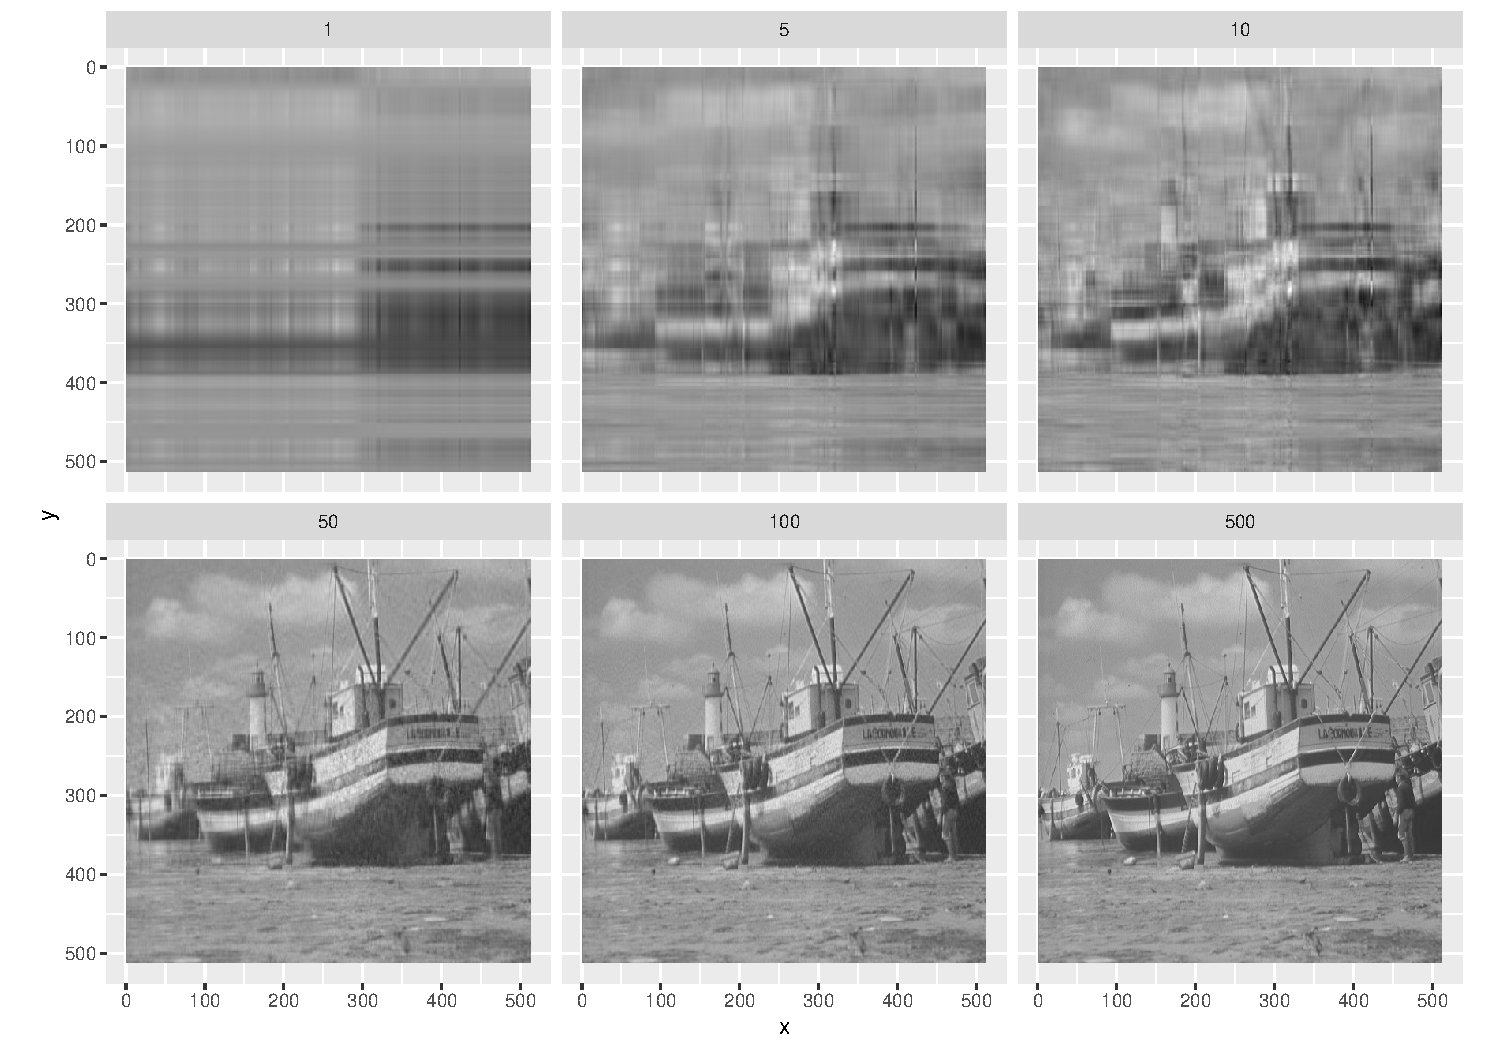
\includegraphics[width=0.7\textwidth,height=\textheight]{008_reducing_data_complexity_files/figure-beamer/unnamed-chunk-25-1.pdf}
\end{center}
\end{frame}

\section{Consumer brand perception
survey}\label{consumer-brand-perception-survey-1}

\begin{frame}[fragile]{}
\phantomsection\label{section-28}
\begin{itemize}
\item
  Principal component analysis (PCA) and perceptual maps

  \begin{itemize}
  \tightlist
  \item
    Applying to the reduced example
  \end{itemize}
\end{itemize}

\tiny

\begin{Shaded}
\begin{Highlighting}[]
\NormalTok{consumer\_brand\_sample\_matrix }\OtherTok{\textless{}{-}}\NormalTok{ consumer\_brand\_sample }\SpecialCharTok{|\textgreater{}} 
  \FunctionTok{select}\NormalTok{(}\SpecialCharTok{{-}}\NormalTok{brand) }\SpecialCharTok{|\textgreater{}}
  \FunctionTok{as.matrix}\NormalTok{()}
\NormalTok{consumer\_brand\_sample\_matrix }\SpecialCharTok{|\textgreater{}} \FunctionTok{head}\NormalTok{()}
\end{Highlighting}
\end{Shaded}

\begin{verbatim}
     perform leader
[1,]       2      4
[2,]       9      6
[3,]       5      6
[4,]       3      3
[5,]       1      5
[6,]       8      6
\end{verbatim}
\end{frame}

\begin{frame}[fragile]{}
\phantomsection\label{section-29}
\begin{itemize}
\item
  Principal component analysis (PCA) and perceptual maps

  \begin{itemize}
  \tightlist
  \item
    \texttt{prcomp} output from R
  \end{itemize}
\end{itemize}

\tiny

\begin{Shaded}
\begin{Highlighting}[]
\NormalTok{consumer\_brand\_sample\_matrix\_pca }\OtherTok{\textless{}{-}}\NormalTok{ consumer\_brand\_sample\_matrix }\SpecialCharTok{|\textgreater{}} 
  \FunctionTok{prcomp}\NormalTok{(}\AttributeTok{center =} \ConstantTok{TRUE}\NormalTok{, }\AttributeTok{scale. =} \ConstantTok{TRUE}\NormalTok{)}
\NormalTok{consumer\_brand\_sample\_matrix\_pca}
\end{Highlighting}
\end{Shaded}

\begin{verbatim}
Standard deviations (1, .., p=2):
[1] 1.1051789 0.8823716

Rotation (n x k) = (2 x 2):
              PC1        PC2
perform 0.7071068  0.7071068
leader  0.7071068 -0.7071068
\end{verbatim}
\end{frame}

\begin{frame}[fragile]{}
\phantomsection\label{section-30}
\begin{itemize}
\item
  Principal component analysis (PCA) and perceptual maps

  \begin{itemize}
  \tightlist
  \item
    Structure of \texttt{prcomp}from R
  \end{itemize}
\end{itemize}

\tiny

\begin{Shaded}
\begin{Highlighting}[]
\NormalTok{consumer\_brand\_sample\_matrix\_pca }\SpecialCharTok{|\textgreater{}} \FunctionTok{str}\NormalTok{()}
\end{Highlighting}
\end{Shaded}

\begin{verbatim}
List of 5
 $ sdev    : num [1:2] 1.105 0.882
 $ rotation: num [1:2, 1:2] 0.707 0.707 0.707 -0.707
  ..- attr(*, "dimnames")=List of 2
  .. ..$ : chr [1:2] "perform" "leader"
  .. ..$ : chr [1:2] "PC1" "PC2"
 $ center  : Named num [1:2] 5.8 4.1
  ..- attr(*, "names")= chr [1:2] "perform" "leader"
 $ scale   : Named num [1:2] 3.19 2.23
  ..- attr(*, "names")= chr [1:2] "perform" "leader"
 $ x       : num [1:10, 1:2] -0.874 1.311 0.424 -0.969 -0.779 ...
  ..- attr(*, "dimnames")=List of 2
  .. ..$ : NULL
  .. ..$ : chr [1:2] "PC1" "PC2"
 - attr(*, "class")= chr "prcomp"
\end{verbatim}
\end{frame}

\begin{frame}[fragile]{}
\phantomsection\label{section-31}
\begin{itemize}
\item
  Principal component analysis (PCA) and perceptual maps

  \begin{itemize}
  \tightlist
  \item
    Extracting scores: principle components space
  \end{itemize}
\end{itemize}

\tiny

\begin{Shaded}
\begin{Highlighting}[]
\NormalTok{scores }\OtherTok{\textless{}{-}}\NormalTok{ consumer\_brand\_sample\_matrix\_pca}\SpecialCharTok{$}\NormalTok{x}
\NormalTok{scores}
\end{Highlighting}
\end{Shaded}

\begin{verbatim}
             PC1         PC2
 [1,] -0.8739101 -0.81059416
 [2,]  1.3107664  0.10776349
 [3,]  0.4241852 -0.77881770
 [4,] -0.9688445 -0.27236914
 [5,] -0.7789757 -1.34881917
 [6,]  1.0891211 -0.11388181
 [7,]  1.8489914  0.01282907
 [8,] -0.4937775  1.46901678
 [9,] -0.1771978  1.15243706
[10,] -1.3803587  0.58243559
\end{verbatim}
\end{frame}

\begin{frame}[fragile]{}
\phantomsection\label{section-32}
\begin{itemize}
\item
  Principal component analysis (PCA) and perceptual maps

  \begin{itemize}
  \tightlist
  \item
    Extracting loadings: map from principle components space back into
    the original space
  \end{itemize}
\end{itemize}

\tiny

\begin{Shaded}
\begin{Highlighting}[]
\NormalTok{loadings }\OtherTok{\textless{}{-}}\NormalTok{ consumer\_brand\_sample\_matrix\_pca}\SpecialCharTok{$}\NormalTok{rotation}
\NormalTok{loadings}
\end{Highlighting}
\end{Shaded}

\begin{verbatim}
              PC1        PC2
perform 0.7071068  0.7071068
leader  0.7071068 -0.7071068
\end{verbatim}
\end{frame}

\begin{frame}[fragile]{}
\phantomsection\label{section-33}
\begin{itemize}
\item
  Principal component analysis (PCA) and perceptual maps

  \begin{itemize}
  \tightlist
  \item
    Extracting loadings: map from principle components space back into
    the original space
  \end{itemize}
\end{itemize}

\tiny

\begin{Shaded}
\begin{Highlighting}[]
\NormalTok{consumer\_brand\_sample\_matrix\_center\_scale }\OtherTok{\textless{}{-}}\NormalTok{ consumer\_brand\_sample\_matrix }\SpecialCharTok{|\textgreater{}} 
  \FunctionTok{scale}\NormalTok{(}\AttributeTok{center =} \ConstantTok{TRUE}\NormalTok{, }\AttributeTok{scale =} \ConstantTok{TRUE}\NormalTok{)}
\NormalTok{consumer\_brand\_sample\_matrix\_center\_scale}
\end{Highlighting}
\end{Shaded}

\begin{verbatim}
         perform      leader
 [1,] -1.1911244 -0.04477113
 [2,]  1.0030521  0.85065153
 [3,] -0.2507630  0.85065153
 [4,] -0.8776706 -0.49248246
 [5,] -1.5045782  0.40294020
 [6,]  0.6895983  0.85065153
 [7,]  1.3165059  1.29836285
 [8,]  0.6895983 -1.38790512
 [9,]  0.6895983 -0.94019379
[10,] -0.5642168 -1.38790512
attr(,"scaled:center")
perform  leader 
    5.8     4.1 
attr(,"scaled:scale")
 perform   leader 
3.190263 2.233582 
\end{verbatim}
\end{frame}

\begin{frame}[fragile]{}
\phantomsection\label{section-34}
\begin{itemize}
\item
  Principal component analysis (PCA) and perceptual maps

  \begin{itemize}
  \tightlist
  \item
    Using matrix multiplication, \texttt{\%*\%}, the original centered
    and scaled data, \(X_{c, s}\), and the loadings, \(L\),
    \texttt{loadings} to obtain the scores, \(S\)
  \end{itemize}
\end{itemize}

\[S = X_{c, s}L\]

\tiny

\begin{Shaded}
\begin{Highlighting}[]
\NormalTok{consumer\_brand\_sample\_matrix\_center\_scale }\SpecialCharTok{\%*\%}\NormalTok{ loadings}
\end{Highlighting}
\end{Shaded}

\begin{verbatim}
             PC1         PC2
 [1,] -0.8739101 -0.81059416
 [2,]  1.3107664  0.10776349
 [3,]  0.4241852 -0.77881770
 [4,] -0.9688445 -0.27236914
 [5,] -0.7789757 -1.34881917
 [6,]  1.0891211 -0.11388181
 [7,]  1.8489914  0.01282907
 [8,] -0.4937775  1.46901678
 [9,] -0.1771978  1.15243706
[10,] -1.3803587  0.58243559
\end{verbatim}
\end{frame}

\begin{frame}[fragile]{}
\phantomsection\label{section-35}
\begin{itemize}
\item
  Principal component analysis (PCA) and perceptual maps

  \begin{itemize}
  \tightlist
  \item
    Recovering original centered and scaled data, \(X\), using loadings,
    \(L\),\footnote<.->{\(L\) is an orthogonal matrix, which means that
      \(L\) is a real square matrix such that \(L^tL = LL^t = I\) where
      \(I\) is the identity matrix.} and scores, \(S\)
  \end{itemize}
\end{itemize}

\[SL^t = X_{c, s}LL^t = X_{c, s}I= X_{c, s}\]

\tiny

\begin{Shaded}
\begin{Highlighting}[]
\NormalTok{(scores }\SpecialCharTok{\%*\%} \FunctionTok{t}\NormalTok{(loadings)) }\SpecialCharTok{|\textgreater{}} \FunctionTok{set\_colnames}\NormalTok{(}\FunctionTok{c}\NormalTok{(}\StringTok{"perform"}\NormalTok{, }\StringTok{"leader"}\NormalTok{))}
\end{Highlighting}
\end{Shaded}

\begin{verbatim}
         perform      leader
 [1,] -1.1911244 -0.04477113
 [2,]  1.0030521  0.85065153
 [3,] -0.2507630  0.85065153
 [4,] -0.8776706 -0.49248246
 [5,] -1.5045782  0.40294020
 [6,]  0.6895983  0.85065153
 [7,]  1.3165059  1.29836285
 [8,]  0.6895983 -1.38790512
 [9,]  0.6895983 -0.94019379
[10,] -0.5642168 -1.38790512
\end{verbatim}
\end{frame}

\begin{frame}[fragile]{}
\phantomsection\label{section-36}
\begin{itemize}
\item
  Principal component analysis (PCA) and perceptual maps

  \begin{itemize}
  \tightlist
  \item
    Reconstructing original centered and scaled data using the first
    principal component, \(X_{c, s, p_1}\)
  \end{itemize}
\end{itemize}

\[S_{p_1}L_{p_1}^t = X_{c, s, p_1}\] \tiny

\begin{Shaded}
\begin{Highlighting}[]
\NormalTok{scores[, }\DecValTok{1}\NormalTok{] }\SpecialCharTok{\%*\%} \FunctionTok{t}\NormalTok{(loadings[, }\DecValTok{1}\NormalTok{])}
\end{Highlighting}
\end{Shaded}

\begin{verbatim}
         perform     leader
 [1,] -0.6179478 -0.6179478
 [2,]  0.9268518  0.9268518
 [3,]  0.2999442  0.2999442
 [4,] -0.6850765 -0.6850765
 [5,] -0.5508190 -0.5508190
 [6,]  0.7701249  0.7701249
 [7,]  1.3074344  1.3074344
 [8,] -0.3491534 -0.3491534
 [9,] -0.1252977 -0.1252977
[10,] -0.9760610 -0.9760610
\end{verbatim}
\end{frame}

\begin{frame}[fragile]{}
\phantomsection\label{section-37}
\begin{itemize}
\item
  Principal component analysis (PCA) and perceptual maps

  \begin{itemize}
  \tightlist
  \item
    Reconstructing original centered data using the first principal
    component, \(X_{c, p_1}\)
  \end{itemize}
\end{itemize}

\tiny

\begin{Shaded}
\begin{Highlighting}[]
\NormalTok{scores[, }\DecValTok{1}\NormalTok{] }\SpecialCharTok{\%*\%} \FunctionTok{t}\NormalTok{(loadings[, }\DecValTok{1}\NormalTok{]) }\SpecialCharTok{|\textgreater{}} 
  \FunctionTok{scale}\NormalTok{(}\AttributeTok{center =} \ConstantTok{FALSE}\NormalTok{, }\AttributeTok{scale =} \DecValTok{1}\SpecialCharTok{/}\NormalTok{consumer\_brand\_sample\_matrix\_pca}\SpecialCharTok{$}\NormalTok{scale)}
\end{Highlighting}
\end{Shaded}

\begin{verbatim}
         perform     leader
 [1,] -1.9714158 -1.3802370
 [2,]  2.9569010  2.0701996
 [3,]  0.9569010  0.6699501
 [4,] -2.1855743 -1.5301747
 [5,] -1.7572574 -1.2302994
 [6,]  2.4569010  1.7201372
 [7,]  4.1710595  2.9202620
 [8,] -1.1138912 -0.7798628
 [9,] -0.3997327 -0.2798628
[10,] -3.1138912 -2.1801123
attr(,"scaled:scale")
  perform    leader 
0.3134538 0.4477113 
\end{verbatim}
\end{frame}

\begin{frame}[fragile]{}
\phantomsection\label{section-38}
\begin{itemize}
\item
  Principal component analysis (PCA) and perceptual maps

  \begin{itemize}
  \tightlist
  \item
    Reconstructing original data using the first principal component,
    \(X_{p_1}\)
  \end{itemize}
\end{itemize}

\tiny

\begin{Shaded}
\begin{Highlighting}[]
\NormalTok{scores[, }\DecValTok{1}\NormalTok{] }\SpecialCharTok{\%*\%} \FunctionTok{t}\NormalTok{(loadings[, }\DecValTok{1}\NormalTok{]) }\SpecialCharTok{|\textgreater{}} 
  \FunctionTok{scale}\NormalTok{(}\AttributeTok{center =} \ConstantTok{FALSE}\NormalTok{, }\AttributeTok{scale =} \DecValTok{1}\SpecialCharTok{/}\NormalTok{consumer\_brand\_sample\_matrix\_pca}\SpecialCharTok{$}\NormalTok{scale) }\SpecialCharTok{|\textgreater{}} 
  \FunctionTok{scale}\NormalTok{(}\AttributeTok{center =} \SpecialCharTok{{-}}\NormalTok{consumer\_brand\_sample\_matrix\_pca}\SpecialCharTok{$}\NormalTok{center, }\AttributeTok{scale =} \ConstantTok{FALSE}\NormalTok{)}
\end{Highlighting}
\end{Shaded}

\begin{verbatim}
       perform   leader
 [1,] 3.828584 2.719763
 [2,] 8.756901 6.170200
 [3,] 6.756901 4.769950
 [4,] 3.614426 2.569825
 [5,] 4.042743 2.869701
 [6,] 8.256901 5.820137
 [7,] 9.971059 7.020262
 [8,] 4.686109 3.320137
 [9,] 5.400267 3.820137
[10,] 2.686109 1.919888
attr(,"scaled:scale")
  perform    leader 
0.3134538 0.4477113 
attr(,"scaled:center")
perform  leader 
   -5.8    -4.1 
\end{verbatim}
\end{frame}

\begin{frame}[fragile]{}
\phantomsection\label{section-39}
\begin{itemize}
\item
  Principal component analysis (PCA) and perceptual maps

  \begin{itemize}
  \tightlist
  \item
    Eingevalues, in this case \texttt{variance}, represent the variance
    explained by each principal component
  \end{itemize}
\end{itemize}

\tiny

\begin{Shaded}
\begin{Highlighting}[]
\NormalTok{eigenvalues }\OtherTok{\textless{}{-}}\NormalTok{ consumer\_brand\_sample\_matrix\_pca }\SpecialCharTok{|\textgreater{}} 
  \FunctionTok{tidy}\NormalTok{(}\AttributeTok{matrix =} \StringTok{"eigenvalues"}\NormalTok{) }\SpecialCharTok{|\textgreater{}} 
  \FunctionTok{mutate}\NormalTok{(}\AttributeTok{variance =}\NormalTok{ std.dev}\SpecialCharTok{\^{}}\DecValTok{2}\NormalTok{, }\AttributeTok{.after =}\NormalTok{ std.dev)}
\NormalTok{eigenvalues}
\end{Highlighting}
\end{Shaded}

\begin{verbatim}
# A tibble: 2 x 5
     PC std.dev variance percent cumulative
  <dbl>   <dbl>    <dbl>   <dbl>      <dbl>
1     1   1.11     1.22    0.611      0.611
2     2   0.882    0.779   0.389      1    
\end{verbatim}
\end{frame}

\begin{frame}[fragile]{}
\phantomsection\label{section-40}
\begin{itemize}
\item
  Principal component analysis (PCA) and perceptual maps

  \begin{itemize}
  \tightlist
  \item
    Eingevalues, in this case \texttt{variance}, represent the variance
    explained by each principal component
  \end{itemize}
\end{itemize}

\tiny

\begin{Shaded}
\begin{Highlighting}[]
\FunctionTok{library}\NormalTok{(ggbiplot)}
\NormalTok{consumer\_brand\_sample\_matrix\_pca }\SpecialCharTok{|\textgreater{}} 
  \FunctionTok{ggscreeplot}\NormalTok{() }\SpecialCharTok{+}
  \FunctionTok{scale\_x\_continuous}\NormalTok{(}\AttributeTok{breaks =} \DecValTok{1}\SpecialCharTok{:}\DecValTok{2}\NormalTok{)}
\end{Highlighting}
\end{Shaded}

\begin{center}
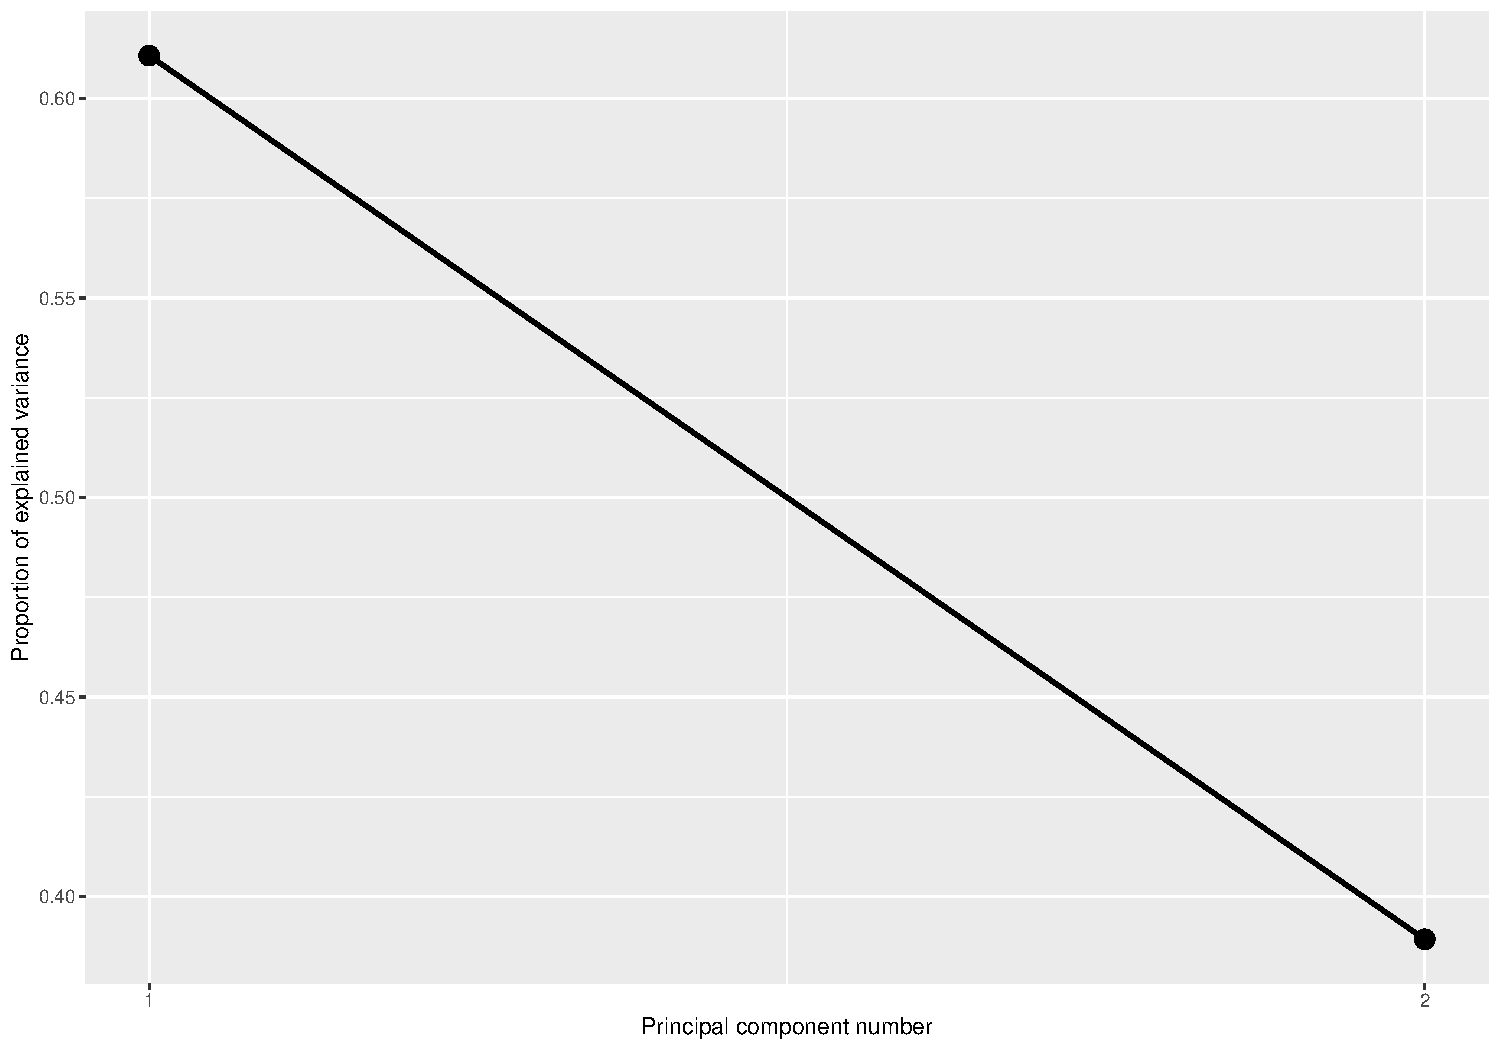
\includegraphics[width=0.5\textwidth,height=\textheight]{008_reducing_data_complexity_files/figure-beamer/unnamed-chunk-38-1.pdf}
\end{center}
\end{frame}

\begin{frame}[fragile]{}
\phantomsection\label{section-41}
\begin{itemize}
\item
  Principal component analysis (PCA) and perceptual maps

  \begin{itemize}
  \item
    A \textbf{biplot} represents visually the scores of the first,
    x-axis, and second, y-axis, of the principal components and the
    corresponding loadings both \textbf{scaled by a
    factor}\footnote<.->{For specific details check out
      \texttt{?stats:::biplot.prcomp}, \texttt{?ggbiplot::ggbiplot} and
      \texttt{?ggbiplot::get\_SVD}}
  \item
    In the case of principal component analysis there are many different
    ways to produce a biplot

    \begin{itemize}
    \tightlist
    \item
      For the differents ways to build a biplot check out
      \href{https://stats.stackexchange.com/questions/141085/positioning-the-arrows-on-a-pca-biplot}{Positioning
      the arrows on a PCA biplot}
    \end{itemize}
  \end{itemize}
\end{itemize}
\end{frame}

\begin{frame}[fragile]{}
\phantomsection\label{section-42}
\begin{itemize}
\item
  Principal component analysis (PCA) and perceptual maps

  \begin{itemize}
  \tightlist
  \item
    Building a biplot using the package \texttt{ggbiplot}
  \end{itemize}
\end{itemize}

\tiny

\begin{Shaded}
\begin{Highlighting}[]
\FunctionTok{ggbiplot}\NormalTok{(}\AttributeTok{pcobj =}\NormalTok{ consumer\_brand\_sample\_matrix\_pca,}
         \AttributeTok{groups =}\NormalTok{ consumer\_brand\_sample}\SpecialCharTok{$}\NormalTok{brand,}
         \AttributeTok{scale =} \DecValTok{1}\NormalTok{, }\AttributeTok{pc.biplot =} \ConstantTok{FALSE}\NormalTok{) }\SpecialCharTok{+}
  \FunctionTok{labs}\NormalTok{(}\AttributeTok{color =} \StringTok{"Brands"}\NormalTok{)}
\end{Highlighting}
\end{Shaded}

\begin{center}
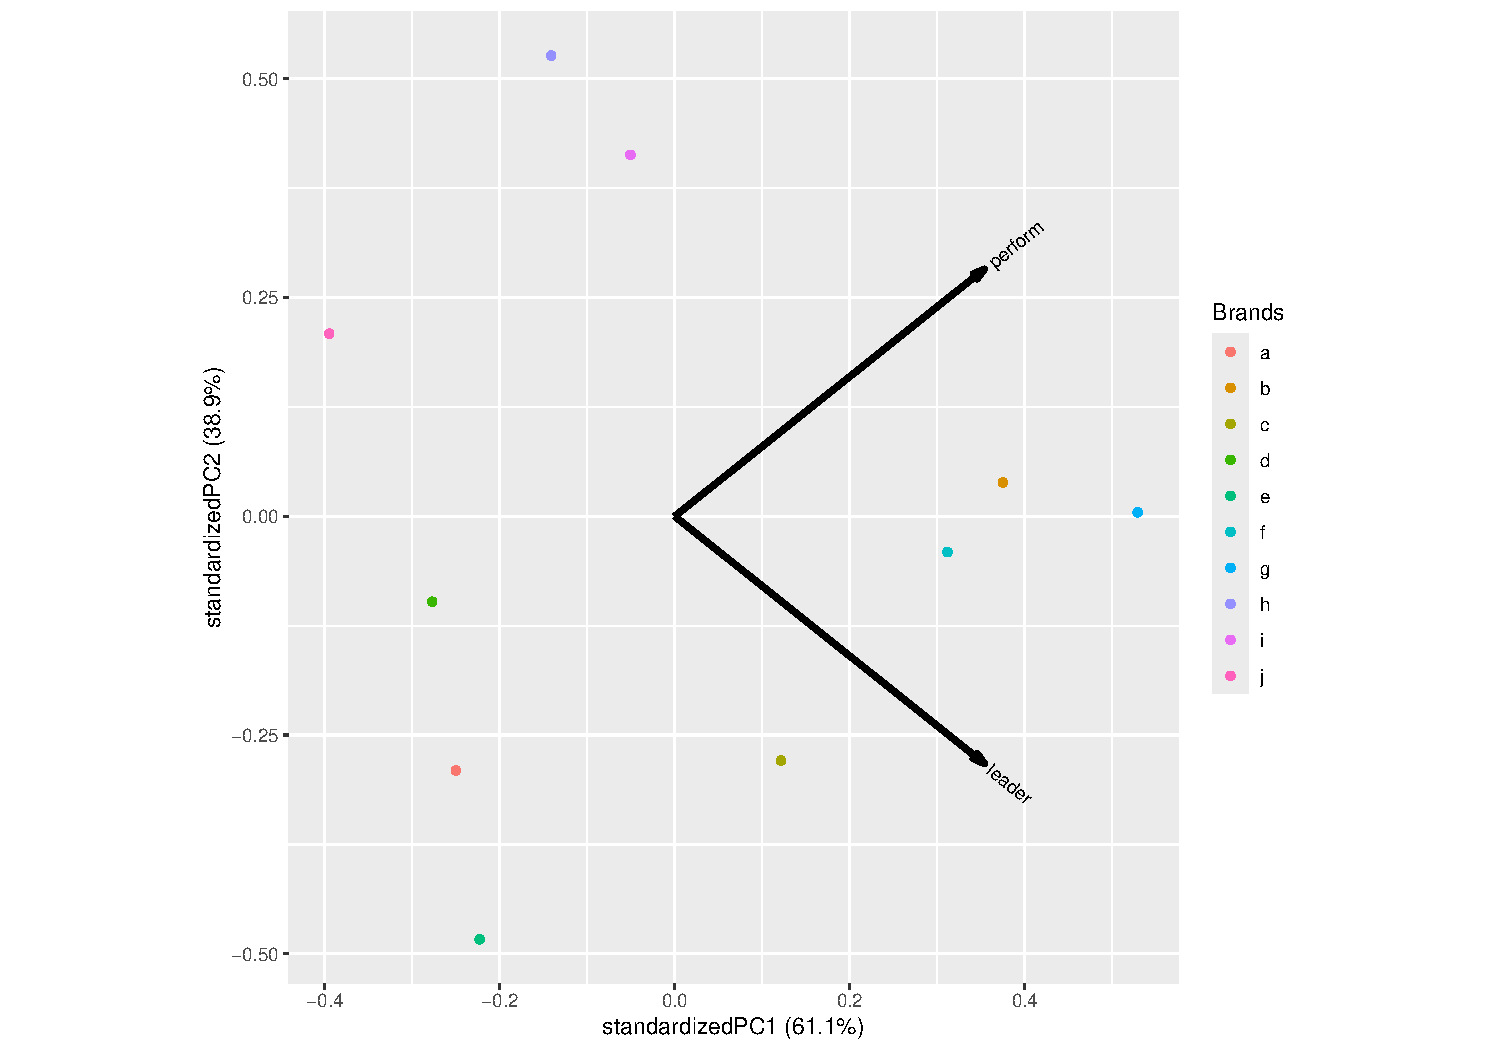
\includegraphics[width=0.5\textwidth,height=\textheight]{008_reducing_data_complexity_files/figure-beamer/unnamed-chunk-39-1.pdf}
\end{center}
\end{frame}

\begin{frame}[fragile]{}
\phantomsection\label{section-43}
\begin{itemize}
\tightlist
\item
  Bibplot for all the consumer brand perception survey
\end{itemize}

\tiny

\begin{Shaded}
\begin{Highlighting}[]
\NormalTok{consumer\_brand\_pca }\OtherTok{\textless{}{-}}\NormalTok{ consumer\_brand }\SpecialCharTok{|\textgreater{}}
  \FunctionTok{select}\NormalTok{(}\SpecialCharTok{{-}}\NormalTok{brand) }\SpecialCharTok{|\textgreater{}} 
  \FunctionTok{prcomp}\NormalTok{(}\AttributeTok{center =} \ConstantTok{TRUE}\NormalTok{, }\AttributeTok{scale. =} \ConstantTok{TRUE}\NormalTok{)}
\NormalTok{consumer\_brand\_pca }\SpecialCharTok{|\textgreater{}} 
  \FunctionTok{ggbiplot}\NormalTok{(}\AttributeTok{groups =}\NormalTok{ consumer\_brand}\SpecialCharTok{$}\NormalTok{brand, }\AttributeTok{scale =} \DecValTok{1}\NormalTok{, }\AttributeTok{pc.biplot =} \ConstantTok{FALSE}\NormalTok{)}
\end{Highlighting}
\end{Shaded}

\begin{center}
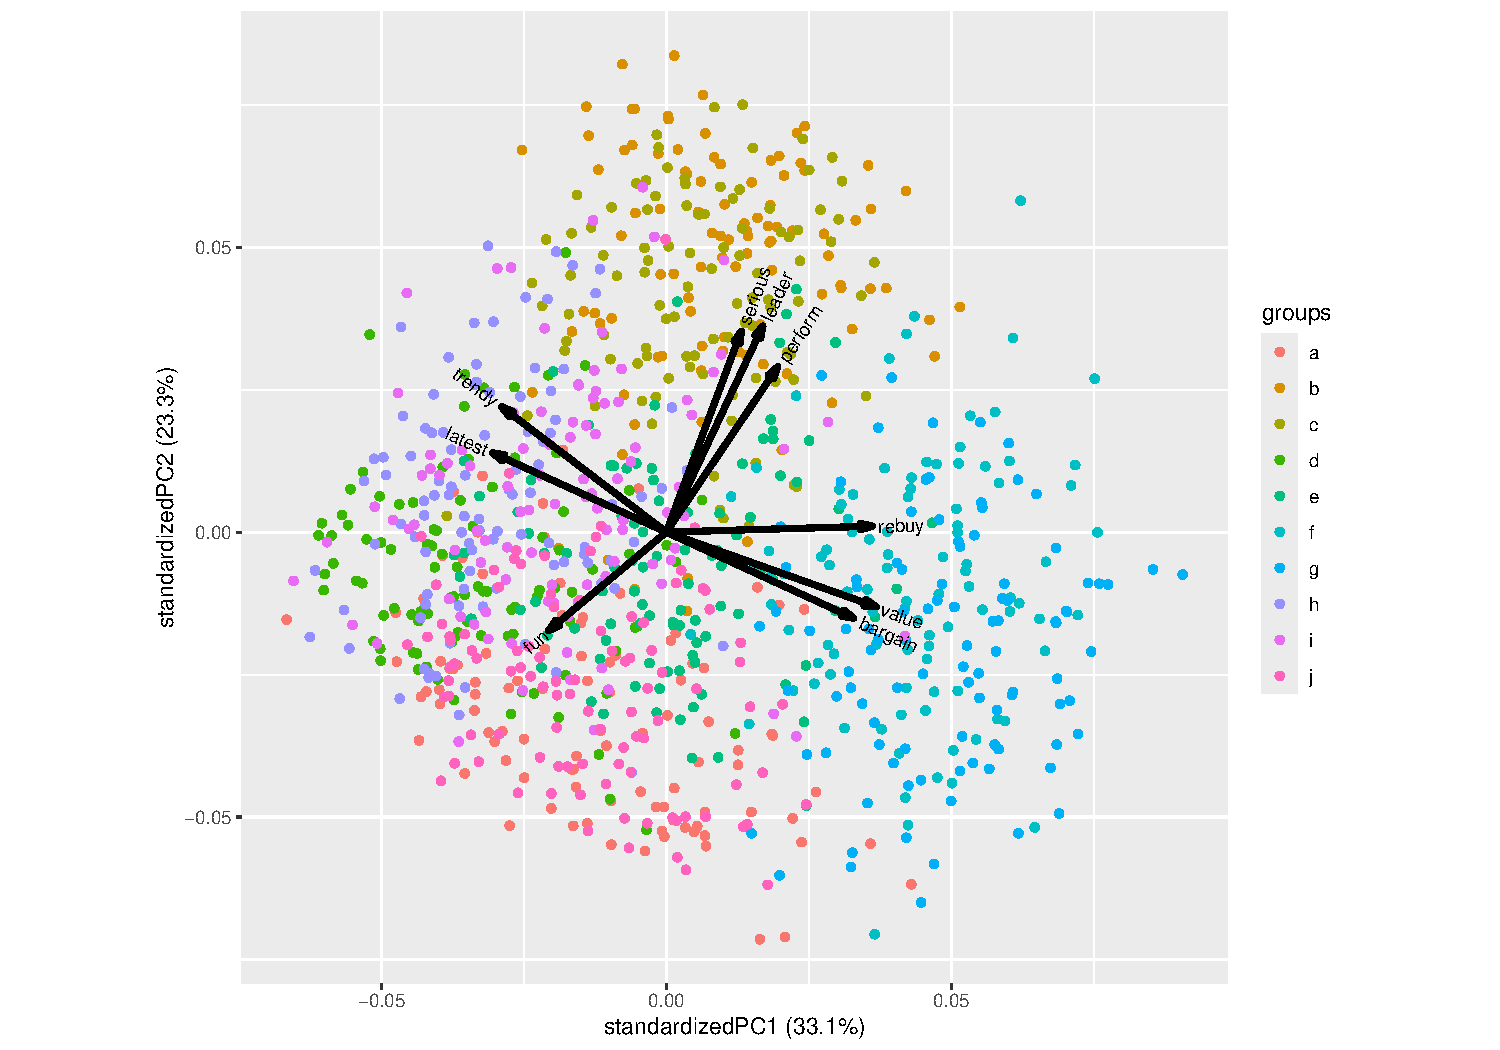
\includegraphics[width=0.5\textwidth,height=\textheight]{008_reducing_data_complexity_files/figure-beamer/unnamed-chunk-40-1.pdf}
\end{center}
\end{frame}

\begin{frame}[fragile]{}
\phantomsection\label{section-44}
\begin{itemize}
\item
  A biplot is a generalization of a scatterplot of 2 variables for the
  case of many variables
  (\citeproc{ref-greenacre_biplots_2010}{Greenacre 2010, 9})
\item
  Variables of the brands that are grouped together are positively
  correlated to each other

  \begin{itemize}
  \tightlist
  \item
    For example \texttt{serious}, \texttt{leader} and \texttt{perform}
    or \texttt{trendy} and \texttt{latest}
  \end{itemize}
\item
  Variables of the brands that are displayed to the opposite sides of
  the biplot origin are negatively correlated to each other

  \begin{itemize}
  \tightlist
  \item
    For example \texttt{fun} in relation to \texttt{serious},
    \texttt{leader} and \texttt{perform} or \texttt{trendy} and
    \texttt{latest} in relation to \texttt{value} and \texttt{bargain}
  \end{itemize}
\end{itemize}
\end{frame}

\begin{frame}[fragile]{}
\phantomsection\label{section-45}
\begin{itemize}
\item
  A biplot is an \textbf{approximated} representation of a data table
  ordered by rows which represents some observations and columns which
  represents some variables

  \begin{itemize}
  \item
    By the term \textbf{approximated} it means that the representation
    is not exact
  \item
    In our case the last biplot was used to represent the data table
    \texttt{consumer\_brand\_sample} by reducing its complexity
  \end{itemize}
\item
  In a biplot the distance between points represent some measure of
  similarity

  \begin{itemize}
  \tightlist
  \item
    In the case of the last biplot for example brand \texttt{g}, that is
    colored in blue, tend to be spatially grouped in the plot
  \end{itemize}
\end{itemize}
\end{frame}

\section{Acknowledgments}\label{acknowledgments}

\begin{frame}{}
\phantomsection\label{section-46}
\begin{itemize}
\item
  To my family that supports me
\item
  To the taxpayers of Colombia and the
  \href{https://www.umng.edu.co/estudiante}{\textbf{UMNG students}} who
  pay my salary
\item
  To the \href{https://www.business-science.io/}{\textbf{Business
  Science}} and \href{https://www.rfordatasci.com/}{\textbf{R4DS Online
  Learning}} communities where I learn
  \href{https://www.r-project.org/about.html}{\textbf{R}} and
  \href{https://www.python.org/about/}{\textbf{\(\pi\)-thon}}
\item
  To the \href{https://www.r-project.org/contributors.html}{\textbf{R
  Core Team}}, the creators of
  \href{https://posit.co/products/open-source/rstudio/}{\textbf{RStudio
  IDE}}, \href{https://quarto.org/}{\textbf{Quarto}} and the authors and
  maintainers of the packages
  \href{https://CRAN.R-project.org/package=tidyverse}{\textbf{tidyverse}},
  \href{https://CRAN.R-project.org/package=skimr}{\textbf{skimr}},
  \href{https://CRAN.R-project.org/package=corrr}{\textbf{corrr}},
  \href{https://CRAN.R-project.org/package=tidyheatmaps}{\textbf{tidyheatmaps}}
  \href{https://CRAN.R-project.org/package=tidymodels}{\textbf{tidymodels}},
  \href{https://CRAN.R-project.org/package=ggforce}{\textbf{ggforce}},
  \href{https://CRAN.R-project.org/package=ggbiplot}{\textbf{ggbiplot}}
  , \href{https://CRAN.R-project.org/package=imager}{\textbf{imager}}
  and
  \href{https://CRAN.R-project.org/package=tinytex}{\textbf{tinytex}}
  for allowing me to access these tools without paying for a license
\item
  To the \href{https://www.kernel.org/category/about.html}{\textbf{Linux
  kernel community}} for allowing me the possibility to use some
  \href{https://static.lwn.net/Distributions/}{\textbf{Linux
  distributions}} as my main
  \href{https://en.wikipedia.org/wiki/Operating_system}{\textbf{OS}}
  without paying for a license
\end{itemize}
\end{frame}

\section*{References}\label{references}
\addcontentsline{toc}{section}{References}

\begin{frame}[allowframebreaks]{References}
\phantomsection\label{refs}
\begin{CSLReferences}{1}{0}
\bibitem[\citeproctext]{ref-chapman_r_2019}
Chapman, Chris, and Elea McDonnell Feit. 2019. \emph{R {For} {Marketing}
{Research} and {Analytics}}. 2nd ed. 2019. Use {R}! Cham: Springer
International Publishing : Imprint: Springer.
\url{https://doi-org.ezproxy.umng.edu.co/10.1007/978-3-030-14316-9}.

\bibitem[\citeproctext]{ref-greenacre_biplots_2010}
Greenacre, Michael J. 2010. \emph{Biplots in Practice}. Bilbao:
Fundación BBVA.
\url{https://www.fbbva.es/microsite/multivariate-statistics/biplots.html}.

\end{CSLReferences}
\end{frame}




\end{document}
